% ============================================================
% Project 2 (PDE BVP) --- LaTeX Report: Direction 3 (Variable Diffusion)
% Build:   latexmk -pdf Method.tex    (pdflatex + bibtex + pdflatex x2)
% ============================================================

\documentclass[11pt,a4paper]{article}



\usepackage[utf8]{inputenc}
\usepackage[T1]{fontenc}
\usepackage{amsmath, amssymb, amsthm}
\usepackage{geometry}
\geometry{a4paper, margin=2.5cm}
\usepackage{graphicx}
\usepackage{booktabs}
\usepackage{array}
\usepackage{listings}
\usepackage{xcolor}
\usepackage{hyperref}
\usepackage{enumitem}
\usepackage{float}
\usepackage{caption}
\usepackage{subcaption}
\usepackage{bm}
\usepackage{algorithm}
\usepackage{algpseudocode}
\usepackage{mdframed}
\usepackage{stmaryrd}


% --- colors ---
\definecolor{lecture}{RGB}{70,130,180}
\definecolor{seminar}{RGB}{205,92,92}
\definecolor{formbg}{RGB}{250,250,245}
\definecolor{formframe}{RGB}{180,170,140}

% --- code listing style (Python) ---
\lstset{
    language=Python,
    basicstyle=\ttfamily\scriptsize,
    keywordstyle=\color{blue}\bfseries,
    commentstyle=\color{green!40!black},
    stringstyle=\color{red!70!black},
    numbers=left,
    numberstyle=\tiny\color{gray},
    frame=single,
    breaklines=true,
    showstringspaces=false,
    tabsize=4,
    captionpos=b,
}

% --- theorem-like environments (course-level set) ---
\newtheorem{theorem}{Theorem}[section]
\newtheorem{lemma}[theorem]{Lemma}
\newtheorem{proposition}[theorem]{Proposition}
\newtheorem{corollary}[theorem]{Corollary}
\theoremstyle{definition}
\newtheorem{definition}[theorem]{Definition}
\newtheorem{assumption}[theorem]{Assumption}
\newtheorem{example}[theorem]{Example}
\theoremstyle{remark}
\newtheorem{remark}[theorem]{Remark}

% --- algorithm style ---
\algrenewcommand{\algorithmicrequire}{\textbf{Input:}}
\algrenewcommand{\algorithmicensure}{\textbf{Output:}}
\algrenewcommand{\algorithmiccomment}[1]{\hfill\textcolor{gray}{\# #1}}

% --- form box (for appendices) ---
\newmdenv[
    backgroundcolor=formbg,
    linecolor=formframe,
    linewidth=0.8pt,
    roundcorner=3pt,
    innermargin=5pt,
    outermargin=5pt,
    innertopmargin=8pt,
    innerbottommargin=8pt
]{formbox}

\title{\textbf{Numerical Solution of Elliptic Boundary Value Problems with Variable and Discontinuous Diffusion Coefficients}\\[2mm]
\large Project 2 (PDE BVP) Report --- Direction 3: Variable Diffusion}
\author{
    Team Q \\
    \small Tianrui Ji, 2361367 \quad Meichen Ding, 2362344 \quad Jingyan Wei, 2361411 \\
    \small Han Liu, 2364393 \quad Jiasheng Xu, 2251640 \\
    \small Department of Applied Mathematics
}
\date{November 6, 2026}

\graphicspath{{figures/}}
\setlength{\emergencystretch}{3em}
\begin{document}
\maketitle

\begin{abstract}
We solve the two-dimensional variable-diffusion boundary value problem
$-\nabla\cdot(a\nabla u)=f$ on the unit square using a conservative five-point
finite-difference method (FDM). A conforming triangular $\mathcal P_1$
finite-element method (FEM) provides a matched depth comparison. With positive
shared face conductances and symmetric Dirichlet elimination, the FDM matrix is
symmetric positive definite and satisfies a discrete maximum principle. On the
smooth manufactured problem $a=1+x$, both methods show approximately second-order
error in nodal and common reconstructed $L^2$ norms over four mesh levels.
For a layered coefficient jump from $1$ to $10$, harmonic face averaging recovers
the exact solution at nodes to round-off, while arithmetic averaging gives a
maximum nodal error of $9.60\times10^{-3}$ at $N=63$ and a maximum interface-flux
error of $0.662$. The latter persists near the prescribed horizontal boundaries
under refinement, even though the arithmetic matrix remains symmetric and its
shared flux is locally conservative. A matched FDM--FEM comparison records errors,
residuals, sparse costs, and solver iterations. Independent validation confirms
the main numerical claims and identifies the limits of the diagnostics.
\end{abstract}

\noindent\textbf{Keywords:} elliptic boundary value problem, variable diffusion, discontinuous coefficients, conservative finite difference method, harmonic averaging, discrete maximum principle, method of manufactured solutions, finite element method

\tableofcontents
\newpage

% ============================================================
\section{Introduction and Motivation}
% ============================================================

\subsection{Problem Background}
Second-order elliptic partial differential equations (PDEs) in divergence form constitute the foundational mathematical framework for modelling steady-state diffusive transport across heterogeneous media \cite{hiptmair2025, quarteroni2017}. In engineering and physical sciences, the governing law arises from combining a universal conservation principle (such as conservation of thermal energy, mass, or electric charge) with a constitutive flux-gradient relation, notably Fourier's law of heat conduction $\bm{j} = -a(x,y)\nabla u$, Fick's law of diffusion, or Darcy's law for single-phase fluid flow in porous formations \cite{hackbusch2017, hiptmair2025}.

In realistic applications---such as thermal management of multi-layered semiconductor packaging, groundwater hydrology through stratified sedimentary rock, or electrostatic field simulation in composite dielectrics---the material diffusivity or conductivity $a(x,y)$ varies spatially and frequently exhibits sharp jump discontinuities across internal material interfaces \cite{quarteroni2017}. Solving these problems numerically presents a fundamental challenge: standard pointwise discretisations of the expanded non-divergence operator $-a\Delta u - \nabla a \cdot \nabla u$ break down at material interfaces where $\nabla a$ is classically undefined. Failing to honour the divergence structure leads to a loss of local flux conservation, destroys the symmetry of the discrete operator, and produces spurious $\mathcal{O}(1)$ errors in the interfacial transport rate. Consequently, designing and verifying conservative numerical schemes that rigorously preserve physical flux continuity and discrete structural invariants (symmetry, positive definiteness, and monotonicity) is essential for reliable scientific computing.

\subsection{Mathematical Model}
We consider the two-dimensional stationary diffusion equation posed on the open unit square domain $\Omega = (0,1)^2 \subset \mathbb{R}^2$ with boundary $\partial\Omega = \Gamma_D$ subject to prescribed Dirichlet boundary conditions:
\begin{equation}
    -\nabla\cdot\bigl(a(x,y)\nabla u(x,y)\bigr) = f(x,y) \quad \text{in } \Omega,
    \qquad
    u(x,y) = g(x,y) \quad \text{on } \partial\Omega,
    \label{eq:bvp}
\end{equation}
where $u: \bar{\Omega} \to \mathbb{R}$ denotes the unknown scalar potential (e.g., temperature or hydraulic head), $f \in L^2(\Omega)$ represents the volumetric source density, and $g \in H^{1/2}(\partial\Omega) \cap C^0(\partial\Omega)$ is the given boundary data. In the special homogeneous, isotropic limit where $a(x,y) \equiv 1$, Equation \eqref{eq:bvp} reduces to the classical Poisson problem:
\begin{equation}
    -\Delta u = f \quad \text{in } \Omega, \qquad u|_{\partial\Omega} = g.
    \label{eq:poisson}
\end{equation}

\begin{assumption}[Uniform Ellipticity and Boundedness]
\label{ass:ellipticity}
The diffusion coefficient $a \in L^\infty(\Omega)$ is uniformly positive and bounded almost everywhere in $\Omega$; that is, there exist constants $a_{\min}, a_{\max} \in \mathbb{R}$ such that
\begin{equation}
    0 < a_{\min} \le a(x,y) \le a_{\max} < \infty \quad \text{for a.e. } (x,y) \in \Omega.
    \label{eq:bounds_a}
\end{equation}
We define the global material contrast ratio as $\varrho_a := a_{\max} / a_{\min} \ge 1$.
\end{assumption}

\paragraph{Divergence Form vs.\ Non-Divergence Form and Interface Conditions.}
When $a \in C^1(\bar{\Omega})$ and $u \in C^2(\Omega) \cap C^0(\bar{\Omega})$, applying the product rule of vector calculus yields the equivalent non-divergence representation:
\begin{equation}
    -\nabla\cdot\bigl(a(x,y)\nabla u\bigr) = -a(x,y)\Delta u - \nabla a(x,y)\cdot\nabla u = f(x,y).
    \label{eq:non_div}
\end{equation}
However, when $\Omega$ is partitioned into two disjoint subdomains $\Omega_1$ and $\Omega_2$ separated by a smooth internal interface $\Sigma = \partial\Omega_1 \cap \partial\Omega_2$ (such as the vertical material interface $\Sigma = \{x = 1/2\}$), the coefficient $a(x,y)$ may have a finite jump discontinuity across $\Sigma$. In this regime, $\nabla a$ involves a Dirac delta distribution supported on $\Sigma$, rendering the pointwise differential operator \eqref{eq:non_div} mathematically invalid. 

To interpret \eqref{eq:bvp} rigorously for piecewise-smooth coefficients, we invoke the integral conservation law $\int_V \nabla\cdot\bm{j}\,dxdy = \int_{\partial V} \bm{j}\cdot\bm{n}\,ds = \int_V f\,dxdy$ over an arbitrary control volume $V \subset \Omega$ straddling $\Sigma$, where $\bm{j}(x,y) := -a(x,y)\nabla u(x,y)$ is the physical diffusive flux. Shrinking $V$ onto the interface $\Sigma$ yields the classical piecewise strong formulation coupled with physical transmission conditions:
\begin{equation}
    \begin{cases}
        -\nabla\cdot(a\nabla u) = f & \text{in } \Omega_1 \cup \Omega_2, \\[1mm]
        \llbracket u \rrbracket_\Sigma := u|_{\Omega_1} - u|_{\Omega_2} = 0 & \text{on } \Sigma \quad \text{(continuity of potential)}, \\[1mm]
        \llbracket -a\nabla u \cdot \bm{n}_\Sigma \rrbracket_\Sigma := \bigl(-a_1\nabla u_1 + a_2\nabla u_2\bigr)\cdot\bm{n}_\Sigma = 0 & \text{on } \Sigma \quad \text{(continuity of normal flux)},
    \end{cases}
    \label{eq:interface_cond}
\end{equation}
where $\bm{n}_\Sigma$ denotes the unit normal vector pointing from $\Omega_1$ into $\Omega_2$. Preserving both conditions in \eqref{eq:interface_cond} is the central mathematical requirement of our numerical discretisation; classical treatments either resolve the interface by the mesh or modify the stencil across it \cite{leveque1994imm}.

\paragraph{Variational Formulation and Well-Posedness.}
Because $a \in L^\infty(\Omega)$ does not admit classical derivatives across interfaces, the natural mathematical setting for \eqref{eq:bvp} is the Sobolev space $H^1(\Omega)$. Let $\tilde{g} \in H^1(\Omega)$ be a continuous lifting (extension) of the Dirichlet boundary data such that $\tilde{g}|_{\partial\Omega} = g$ in the trace sense, and decompose the solution as $u = u_0 + \tilde{g}$, where $u_0 \in H_0^1(\Omega) := \{v \in H^1(\Omega) : v|_{\partial\Omega} = 0\}$. Multiplying \eqref{eq:bvp} by an arbitrary test function $v \in H_0^1(\Omega)$ and applying Green's first identity over $\Omega_1$ and $\Omega_2$ yields:
\begin{equation}
    \int_\Omega a(x,y)\nabla u \cdot \nabla v \, dxdy - \int_{\partial\Omega} a\partial_n u \, v \, ds + \int_\Sigma \llbracket -a\nabla u \cdot \bm{n}_\Sigma \rrbracket_\Sigma v \, ds = \int_\Omega f v \, dxdy.
    \label{eq:green_split}
\end{equation}
Since $v=0$ on $\partial\Omega$, the outer-boundary term vanishes.
For a piecewise-smooth exact solution, comparison with the weak formulation
shows that the interface flux jump must vanish in the trace sense. This is
the continuous transmission condition. A conforming Galerkin method enforces
the weak equations only for its finite-dimensional test functions; its raw
piecewise-linear element fluxes may still jump. The fitted-mesh method below
requires no explicit interface multiplier.

We thus arrive at the standard weak formulation: find $u_0 \in H_0^1(\Omega)$ such that
\begin{equation}
    \mathcal{B}(u_0, v) = \ell(v) - \mathcal{B}(\tilde{g}, v) \qquad \forall v \in H_0^1(\Omega),
    \label{eq:weak_form}
\end{equation}
where the bilinear form $\mathcal{B}(\cdot,\cdot): H_0^1(\Omega) \times H_0^1(\Omega) \to \mathbb{R}$ and linear functional $\ell: H_0^1(\Omega) \to \mathbb{R}$ are defined by
\begin{equation}
    \mathcal{B}(w, v) := \int_\Omega a(x,y)\nabla w \cdot \nabla v \, dxdy, \qquad \ell(v) := \int_\Omega f(x,y) v(x,y) \, dxdy.
    \label{eq:bilinear_def}
\end{equation}

\begin{theorem}[Well-Posedness and A Priori Stability Estimate]
\label{thm:well_posed}
Suppose Assumption \ref{ass:ellipticity} holds, $f \in L^2(\Omega)$, and $g \in H^{1/2}(\partial\Omega)$. Then the weak formulation \eqref{eq:weak_form} admits a unique solution $u \in H^1(\Omega)$ with $u - \tilde{g} \in H_0^1(\Omega)$. Moreover, for homogeneous Dirichlet data ($g = 0$), the solution satisfies the a priori stability bound
\begin{equation}
    \|\nabla u\|_{L^2(\Omega)} \le \frac{C_P}{a_{\min}} \|f\|_{L^2(\Omega)}, \qquad \|u\|_{H^1(\Omega)} \le \frac{C_P\sqrt{1+C_P^2}}{a_{\min}} \|f\|_{L^2(\Omega)},
    \label{eq:apriori_bound}
\end{equation}
where $C_P > 0$ is the Poincaré constant of the domain $\Omega = (0,1)^2$.
\end{theorem}

\begin{proof}
We verify the hypotheses of the Lax--Milgram Lemma \cite{quarteroni2017} on the Hilbert space $V = H_0^1(\Omega)$ equipped with the full norm $\|v\|_{H^1(\Omega)} = (\|v\|_{L^2(\Omega)}^2 + \|\nabla v\|_{L^2(\Omega)}^2)^{1/2}$:
\begin{enumerate}[label=(\roman*), leftmargin=2em, itemsep=2pt]
    \item \emph{Continuity of $\mathcal{B}(\cdot,\cdot)$:} By the Cauchy--Schwarz inequality and the upper bound in \eqref{eq:bounds_a}, for all $w, v \in H_0^1(\Omega)$,
    \begin{align*}
        |\mathcal{B}(w,v)|
        &\le \int_\Omega |a(x,y)|\,|\nabla w\cdot\nabla v|\,dxdy
         \le a_{\max}\|\nabla w\|_{L^2(\Omega)}\|\nabla v\|_{L^2(\Omega)} \\
        &\le a_{\max}\|w\|_{H^1(\Omega)}\|v\|_{H^1(\Omega)}.
    \end{align*}
    \item \emph{Coercivity of $\mathcal{B}(\cdot,\cdot)$:} Recall the Poincaré--Friedrichs inequality on $H_0^1(\Omega)$: there exists $C_P > 0$ (specifically $C_P = 1/(\sqrt{2}\pi)$ on $(0,1)^2$) such that $\|v\|_{L^2(\Omega)} \le C_P \|\nabla v\|_{L^2(\Omega)}$ for all $v \in H_0^1(\Omega)$. Consequently, $\|v\|_{H^1(\Omega)}^2 \le (1 + C_P^2)\|\nabla v\|_{L^2(\Omega)}^2$. Using the lower bound in \eqref{eq:bounds_a}, we obtain
    \[
        \mathcal{B}(v,v) = \int_\Omega a(x,y)|\nabla v|^2 \, dxdy \ge a_{\min} \|\nabla v\|_{L^2(\Omega)}^2 \ge \frac{a_{\min}}{1 + C_P^2} \|v\|_{H^1(\Omega)}^2 =: \alpha \|v\|_{H^1(\Omega)}^2.
    \]
    \item \emph{Boundedness of the right-hand side:} By the Cauchy--Schwarz and Poincaré inequalities, $|\ell(v)| \le \|f\|_{L^2(\Omega)} \|v\|_{L^2(\Omega)} \le C_P \|f\|_{L^2(\Omega)} \|\nabla v\|_{L^2(\Omega)}$, and $|\mathcal{B}(\tilde{g}, v)| \le a_{\max} \|\tilde{g}\|_{H^1(\Omega)} \|v\|_{H^1(\Omega)}$.
\end{enumerate}
By the Lax--Milgram Lemma, a unique weak solution exists. Setting $v = u \in H_0^1(\Omega)$ when $g = 0$ gives $a_{\min}\|\nabla u\|_{L^2(\Omega)}^2 \le \mathcal{B}(u,u) = \ell(u) \le C_P \|f\|_{L^2(\Omega)} \|\nabla u\|_{L^2(\Omega)}$, which immediately yields \eqref{eq:apriori_bound}.
\end{proof}

\begin{remark}[Continuous Maximum Principle]
\label{rem:cmp}
In addition to $H^1$ stability, the divergence-form elliptic operator satisfies a weak maximum principle \cite{hackbusch2017}: when the source term vanishes ($f \equiv 0$ in $\Omega$), the weak solution $u \in H^1(\Omega) \cap C^0(\bar{\Omega})$ attains its extrema on the boundary $\partial\Omega$, satisfying
\begin{equation}
    \min_{\partial\Omega} g \le u(x,y) \le \max_{\partial\Omega} g \qquad \forall (x,y) \in \bar{\Omega}.
    \label{eq:cmp}
\end{equation}
In Section~2.4, we prove that our conservative finite difference scheme preserves an exact discrete analogue of \eqref{eq:cmp} via its M-matrix sign structure.
\end{remark}

\subsection{Overview of the Report}
The remainder of this report is structured as follows. In Section 2, we derive the conservative five-point finite difference scheme from local control-volume flux balances, establish the second-order truncation error for smooth coefficients, derive the resistor-in-series harmonic averaging formula for discontinuous interfaces, and rigorously prove the symmetry, positive definiteness, and M-matrix properties of the assembled algebraic system. Section 3 details our sparse matrix implementation, algorithmic vectorisation in \texttt{scipy.sparse}, and solver selection criteria. Section 4 presents our comprehensive verification campaign---including the smooth Method of Manufactured Solutions (MMS) benchmark, algebraic-versus-discretisation error separation, the stratified discontinuous interface benchmark, conditioning sensitivity to coefficient contrast, and a matched-setting depth comparison against $\mathcal{P}_1$ finite elements. Finally, Section 5 summarises our main findings and discusses structural limitations.




\newpage
% ============================================================
\section{Discretisation and Analysis}
% ============================================================

\subsection{Discrete Scheme}
To discretise the divergence-form elliptic boundary value problem \eqref{eq:bvp} while strictly honouring the local conservation law, we employ a vertex-centred (node-centred) conservative finite-volume discretisation, written in finite-difference form, derived via the finite volume balance principle \cite{hackbusch2017, hiptmair2025}.

\paragraph{Uniform Mesh and Dual Control Volumes.}
Let $N \in \mathbb{N}$ ($N \ge 2$) denote the number of subintervals along each coordinate axis, defining a uniform Cartesian mesh of spacing $h := 1/N$. Let $n := N - 1$ be the number of interior grid points per spatial direction. The set of all grid nodes on $\bar{\Omega} = [0,1]^2$ is given by
\begin{equation}
	\bar{\Omega}_h := \bigl\{ \bm{x}_{ij} = (x_i, y_j) = (ih, jh) : 0 \le i, j \le N \bigr\},
	\label{eq:mesh_def}
\end{equation}
which partitions into the interior node set $\Omega_h := \{ \bm{x}_{ij} \in \bar{\Omega}_h : 1 \le i, j \le n \}$ of cardinality $n^2$ and the boundary node set $\Gamma_h := \bar{\Omega}_h \setminus \Omega_h$. Around each interior node $\bm{x}_{ij} \in \Omega_h$, we construct the dual square control volume (cell)
\begin{equation}
	K_{ij} := \bigl[x_{i-1/2}, x_{i+1/2}\bigr] \times \bigl[y_{j-1/2}, y_{j+1/2}\bigr], \qquad \text{with } x_{i\pm 1/2} := x_i \pm \frac{h}{2}, \quad y_{j\pm 1/2} := y_j \pm \frac{h}{2},
	\label{eq:control_vol}
\end{equation}
whose area is $|K_{ij}| = h^2$ and whose boundary $\partial K_{ij} = \gamma_{ij}^E \cup \gamma_{ij}^W \cup \gamma_{ij}^N \cup \gamma_{ij}^S$ consists of four straight cell faces of length $h$ centred at the staggered midpoints $\bm{x}_{i+1/2,j}$ (East), $\bm{x}_{i-1/2,j}$ (West), $\bm{x}_{i,j+1/2}$ (North), and $\bm{x}_{i,j-1/2}$ (South).

\paragraph{Flux Balance and Five-Point Stencil Derivation.}
Integrating the governing PDE \eqref{eq:bvp} over the control volume $K_{ij}$ and applying the Gauss divergence theorem yields the exact local balance identity:
\begin{equation}
	\int_{K_{ij}} -\nabla\cdot\bigl(a(x,y)\nabla u\bigr)\,dxdy = \int_{\partial K_{ij}} \bm{j}\cdot\bm{n}\,ds = \int_{K_{ij}} f(x,y)\,dxdy,
	\label{eq:fv_balance}
\end{equation}
where $\bm{j} = -a\nabla u$ is the diffusive flux and $\bm{n}$ is the outward unit normal on $\partial K_{ij}$. Approximating the cell source integral by the midpoint quadrature rule $\int_{K_{ij}} f\,dxdy \approx h^2 f_{ij}$ with $f_{ij} := f(x_i,y_j)$, and decomposing the boundary integral over the four faces gives
\begin{equation}
	\frac{1}{h}\bigl(F_{i+1/2,j} - F_{i-1/2,j}\bigr) + \frac{1}{h}\bigl(G_{i,j+1/2} - G_{i,j-1/2}\bigr) = f_{ij},
	\label{eq:discrete_balance}
\end{equation}
where $F_{i\pm 1/2,j} \approx \frac{1}{h}\int_{\gamma_{ij}^{E/W}} (-a\partial_x u)\,dy$ and $G_{i,j\pm 1/2} \approx \frac{1}{h}\int_{\gamma_{ij}^{N/S}} (-a\partial_y u)\,dx$ denote the face-averaged numerical fluxes in the $+x$ and $+y$ directions, respectively; the net outward flux through $\partial K_{ij}$ is then $h(F_{i+1/2,j}-F_{i-1/2,j}) + h(G_{i,j+1/2}-G_{i,j-1/2})$. Let $U_{ij} \approx u(x_i, y_j)$ denote the discrete nodal approximation. Replacing the normal derivatives at the cell faces with centred two-point finite difference quotients scaled by effective face conductances, we define the numerical fluxes:
\begin{align}
	F_{i+1/2,j} &:= -a_{i+1/2,j}\frac{U_{i+1,j} - U_{ij}}{h}, & F_{i-1/2,j} &:= -a_{i-1/2,j}\frac{U_{ij} - U_{i-1,j}}{h}, \label{eq:flux_x} \\
	G_{i,j+1/2} &:= -a_{i,j+1/2}\frac{U_{i,j+1} - U_{ij}}{h}, & G_{i,j-1/2} &:= -a_{i,j-1/2}\frac{U_{ij} - U_{i,j-1}}{h}. \label{eq:flux_y}
\end{align}
For compactness, at node $(i,j)$ we denote the four local face coefficients by $a_E := a_{i+1/2,j}$, $a_W := a_{i-1/2,j}$, $a_N := a_{i,j+1/2}$, and $a_S := a_{i,j-1/2}$. Substituting \eqref{eq:flux_x}--\eqref{eq:flux_y} into \eqref{eq:discrete_balance} yields the conservative five-point finite difference operator $A_h$:
\begin{equation}
	(A_h U)_{ij} := \frac{1}{h^2}\Bigl[ a_E(U_{ij} - U_{i+1,j}) + a_W(U_{ij} - U_{i-1,j}) + a_N(U_{ij} - U_{i,j+1}) + a_S(U_{ij} - U_{i,j-1}) \Bigr] = f_{ij}.
	\label{eq:conservative_fdm}
\end{equation}
Collecting terms with respect to the five nodal values in the stencil shows that row $(i,j)$ takes the form
\begin{equation}
	(A_h U)_{ij} = \frac{1}{h^2}\Bigl[ (a_E + a_W + a_N + a_S)U_{ij} - a_W U_{i-1,j} - a_E U_{i+1,j} - a_S U_{i,j-1} - a_N U_{i,j+1} \Bigr] = f_{ij}.
	\label{eq:stencil_collected}
\end{equation}
In difference-star (stencil) notation \cite{hackbusch2017}, the discrete operator at node $(i,j)$ is represented as
\begin{equation}
	A_h\big|_{(i,j)} = \frac{1}{h^2}
	\begin{bmatrix}
		0 & -a_{i,j+1/2} & 0 \\[1mm]
		-a_{i-1/2,j} & a_\Sigma^{(i,j)} & -a_{i+1/2,j} \\[1mm]
		0 & -a_{i,j-1/2} & 0
	\end{bmatrix},
	\label{eq:stencil_star}
\end{equation}
where $a_\Sigma^{(i,j)} := a_{i+1/2,j} + a_{i-1/2,j} + a_{i,j+1/2} + a_{i,j-1/2}$ denotes the sum of the four face conductances, so that the interior row sums of $A_h$ vanish.

\begin{example}[Reduction to the Standard Five-Point Laplacian Stencil]
	In the homogeneous Poisson limit $a(x,y) \equiv 1$, all face conductances equal unity ($a_E = a_W = a_N = a_S = 1$ and $a_\Sigma^{(i,j)} = 4$). Equation \eqref{eq:stencil_collected} reduces identically to the classical five-point discrete Laplacian operator. For any $w \in C^6(\bar{\Omega})$ the operator applied to the \emph{exact} nodal values reads
	\begin{equation}
		(A_h w)_{ij} = \frac{4w_{ij} - w_{i-1,j} - w_{i+1,j} - w_{i,j-1} - w_{i,j+1}}{h^2} = -\Delta w(x_i,y_j) + \mathcal{O}(h^2),
		\label{eq:poisson_stencil}
	\end{equation}
so that $A_h$ is a second-order approximation of $-\Delta$. Note that the discrete unknown satisfies $U_{ij} = u(x_i,y_j) + \mathcal{O}(h^2)$ only, so the two must not be identified.
\end{example}

\paragraph{Grid-to-Vector Index Mapping and Sparsity Structure.}
To assemble \eqref{eq:stencil_collected} into a matrix-vector algebraic system $A_h \bm{u} = \bm{b}$ over the $n^2$ interior unknowns, we establish a bijective grid-to-vector ordering map. Following the `indexing='ij'` convention (where axis $0$ corresponds to $x_i$ and axis $1$ corresponds to $y_j$, so that $y$ varies fastest within each vertical grid line $x_i$), we define the zero-based row-major lexicographical index map $\phi: \{1,\dots,n\}^2 \to \{0,1,\dots,n^2-1\}$ by
\begin{equation}
	k = \phi(i,j) := (i-1)n + (j-1), \qquad 1 \le i,j \le n.
	\label{eq:index_map}
\end{equation}
In Python zero-based interior grid coordinates $(i_0, j_0) := (i-1, j-1) \in \{0,\dots,n-1\}^2$, Equation \eqref{eq:index_map} reads simply $k = i_0 n + j_0$. The inverse mapping $\phi^{-1}(k)$ uniquely recovers the two-dimensional spatial indices via integer division and modulo arithmetic \cite{quarteroni2017}:
\begin{equation}
	i = \lfloor k / n \rfloor + 1, \qquad j = (k \bmod n) + 1, \qquad 0 \le k \le n^2 - 1.
	\label{eq:inverse_map}
\end{equation}
Under this ordering, an interior node $(i,j)$ at global row index $k = \phi(i,j)$ couples to its four cardinal neighbours at column indices:
\begin{equation}
	\phi(i, j\pm 1) = k \pm 1 \quad (\text{North/South}), \qquad \phi(i\pm 1, j) = k \pm n \quad (\text{East/West}).
	\label{eq:neighbour_offsets}
\end{equation}
Consequently, the global stiffness matrix $A_h \in \mathbb{R}^{n^2 \times n^2}$ exhibits a symmetric block-tridiagonal structure partitioned into $n \times n$ blocks of size $n \times n$ each:
\begin{equation}
	A_h = \frac{1}{h^2}
	\begin{bmatrix}
		T_1 & -D_{1,2} & 0 & \cdots & 0 \\
		-D_{1,2} & T_2 & -D_{2,3} & \ddots & \vdots \\
		0 & -D_{2,3} & \ddots & \ddots & 0 \\
		\vdots & \ddots & \ddots & T_{n-1} & -D_{n-1,n} \\
		0 & \cdots & 0 & -D_{n-1,n} & T_n
	\end{bmatrix},
	\label{eq:block_tridiag}
\end{equation}
where each diagonal block $T_i \in \mathbb{R}^{n \times n}$ ($1 \le i \le n$) is itself a symmetric tridiagonal matrix encoding the vertical ($y$-direction) couplings along grid line $x_i$:
\begin{equation}
	(T_i)_{j,j} = a_\Sigma^{(i,j)}, \qquad (T_i)_{j,j+1} = (T_i)_{j+1,j} = -a_{i,j+1/2} \quad (1 \le j \le n-1),
	\label{eq:Ti_def}
\end{equation}
and each off-diagonal block $D_{i,i+1} \in \mathbb{R}^{n \times n}$ ($1 \le i \le n-1$) is a positive diagonal matrix encoding the horizontal ($x$-direction) face conductances between grid lines $x_i$ and $x_{i+1}$:
\begin{equation}
	D_{i,i+1} = \operatorname{diag}\bigl(a_{i+1/2,1},\, a_{i+1/2,2},\, \dots,\, a_{i+1/2,n}\bigr).
	\label{eq:Di_def}
\end{equation}
Every row of $A_h$ contains at most $5$ non-zero entries (located at offsets $0, \pm 1, \pm n$ from the main diagonal). Accounting for boundary-adjacent rows where exterior couplings are transferred to the right-hand side vector $\bm{b}$, the exact number of non-zero entries in $A_h$ is
\begin{equation}
	\operatorname{nnz}(A_h) = n^2 + 4n(n-1) = 5n^2 - 4n = \mathcal{O}(n^2),
	\label{eq:nnz_count}
\end{equation}
yielding a sparsity density of $\operatorname{nnz}(A_h)/n^4 \sim 5/n^2 \to 0$ as $n \to \infty$. Storing $A_h$ in compressed sparse row (CSR) format reduces both memory complexity and matrix-vector multiplication cost from $\mathcal{O}(n^4)$ to $\mathcal{O}(n^2)$; all sparse algebra in this report is carried out through SciPy's \texttt{scipy.sparse} interface \cite{virtanen2020scipy, harris2020numpy}.

% ------------------------------------------------------------
\subsection{Consistency, Truncation Error, and Interface Conductance}
The accuracy and physical fidelity of the conservative scheme \eqref{eq:conservative_fdm} depend critically on how the face conductances $a_{i\pm 1/2,j}$ and $a_{i,j\pm 1/2}$ are constructed in smooth versus discontinuous regimes.

\paragraph{Taylor Expansion and Second-Order Consistency for Smooth Coefficients.}
Let $\mathcal{L}u := -\nabla\cdot(a\nabla u)$ denote the continuous differential operator. For any sufficiently smooth function $w \in C^6(\bar{\Omega})$, the local truncation error (LTE) at an interior node $\bm{x}_{ij} \in \Omega_h$ is defined as the residual left by substituting the exact nodal values $w_{ij} = w(x_i,y_j)$ into the discrete operator:
\begin{equation}
	\tau_{ij}(w) := (A_h w)_{ij} - (\mathcal{L}w)(x_i,y_j).
	\label{eq:lte_def}
\end{equation}
In regions where $a(x,y)$ is smooth, the face coefficient at $\bm{x}_{i+1/2,j}$ can be evaluated either by direct midpoint sampling $a_{i+1/2,j}^{\text{mid}} := a(x_{i+1/2}, y_j)$ or by arithmetic averaging of adjacent nodal values:
\begin{equation}
	a_{i+1/2,j}^{\text{arith}} := \frac{a(x_i, y_j) + a(x_{i+1}, y_j)}{2}.
	\label{eq:arith_def}
\end{equation}

\begin{theorem}[Second-Order Local Truncation Error in Smooth Regimes]
	\label{thm:truncation_smooth}
	Suppose $a \in C^5(\bar{\Omega})$ and the exact solution satisfies $u \in C^6(\bar{\Omega})$. Then under either exact midpoint evaluation $a_{i\pm 1/2,j} = a(x_{i\pm 1/2},y_j)$ or arithmetic averaging \eqref{eq:arith_def}, the conservative five-point scheme \eqref{eq:conservative_fdm} is second-order consistent with \eqref{eq:bvp}. Specifically, for all $\bm{x}_{ij} \in \Omega_h$,
	\begin{equation}
		\tau_{ij}(u) = \mathcal{O}(h^2) \quad \text{as } h \to 0, \qquad \text{with} \quad \|\bm{\tau}(u)\|_\infty \le C_{\text{LTE}} h^2,
		\label{eq:lte_order2}
	\end{equation}
	where $C_{\text{LTE}} > 0$ depends only on $\|a\|_{C^5(\bar{\Omega})}$ and $\|u\|_{C^6(\bar{\Omega})}$.
\end{theorem}

\begin{proof}
	By linearity and coordinate symmetry, it suffices to analyse the $x$-direction conservative difference operator $\mathcal{D}_x^h u_{ij} := \frac{1}{h}\bigl[ a_{i+1/2,j}\frac{u_{i+1,j}-u_{ij}}{h} - a_{i-1/2,j}\frac{u_{ij}-u_{i-1,j}}{h} \bigr]$ at a fixed $y_j$. Suppressing the index $j$ and expanding $u(x_i+h)$ and $u(x_i)$ in Taylor series about the half-point $x_{i+1/2} = x_i + h/2$ (with step $\delta = h/2$) gives
	\begin{align}
		u(x_{i+1/2} + \delta) &= u_{i+1/2} + \delta u_x\big|_{i+1/2} + \frac{\delta^2}{2}u_{xx}\big|_{i+1/2} + \frac{\delta^3}{6}u_{xxx}\big|_{i+1/2} + \frac{\delta^4}{24}u_{xxxx}\big|_{i+1/2} + \mathcal{O}(h^5), \\
		u(x_{i+1/2} - \delta) &= u_{i+1/2} - \delta u_x\big|_{i+1/2} + \frac{\delta^2}{2}u_{xx}\big|_{i+1/2} - \frac{\delta^3}{6}u_{xxx}\big|_{i+1/2} + \frac{\delta^4}{24}u_{xxxx}\big|_{i+1/2} + \mathcal{O}(h^5).
	\end{align}
	Subtracting the two expansions cancels all even powers of $\delta$, yielding the central difference approximation of the first derivative at $x_{i+1/2}$:
	\begin{equation}
		\frac{u_{i+1} - u_i}{h} = \frac{u(x_{i+1/2}+\delta) - u(x_{i+1/2}-\delta)}{2\delta} = u_x\big|_{i+1/2} + \frac{h^2}{24}u_{xxx}\big|_{i+1/2} + \mathcal{O}(h^4).
		\label{eq:taylor_ux}
	\end{equation}
	Similarly, expanding $a(x_i)$ and $a(x_{i+1})$ about $x_{i+1/2}$ shows that the arithmetic average \eqref{eq:arith_def} satisfies
	\begin{equation}
		a_{i+1/2}^{\text{arith}} = \frac{a(x_{i+1/2}-\delta) + a(x_{i+1/2}+\delta)}{2} = a(x_{i+1/2}) + \frac{h^2}{8}a_{xx}\big|_{i+1/2} + \mathcal{O}(h^4).
		\label{eq:taylor_a_arith}
	\end{equation}
	Thus we may write $a_{i+1/2} = a(x_{i+1/2}) + \theta \frac{h^2}{8}a_{xx}|_{i+1/2} + \mathcal{O}(h^4)$, where $\theta = 0$ for exact midpoint evaluation and $\theta = 1$ for arithmetic averaging. Multiplying $a_{i+1/2}$ by \eqref{eq:taylor_ux} gives the numerical flux expansion at $x_{i+1/2}$:
	\begin{equation}
		a_{i+1/2}\frac{u_{i+1}-u_i}{h} = (au_x)\big|_{i+1/2} + h^2 \psi(x_{i+1/2}) + \mathcal{O}(h^4), \qquad \psi := \frac{1}{24}a u_{xxx} + \frac{\theta}{8}a_{xx}u_x.
		\label{eq:flux_taylor}
	\end{equation}
	Analogously, at $x_{i-1/2}$ we have $a_{i-1/2}\frac{u_i-u_{i-1}}{h} = (au_x)|_{i-1/2} + h^2 \psi(x_{i-1/2}) + \mathcal{O}(h^4)$. Taking the outer central difference of \eqref{eq:flux_taylor} across $[x_{i-1/2}, x_{i+1/2}]$ centered at $x_i$ and applying \eqref{eq:taylor_ux} to the smooth flux function $q(x) := a(x)u_x(x)$ and to $\psi(x)$ yields
	\begin{align}
		\mathcal{D}_x^h u_i &= \frac{q(x_i + h/2) - q(x_i - h/2)}{h} + h^2 \frac{\psi(x_i + h/2) - \psi(x_i - h/2)}{h} + \mathcal{O}(h^3) \nonumber \\
		&= \partial_x(au_x)\big|_{x_i} + \frac{h^2}{24}\partial_x^3(au_x)\big|_{x_i} + h^2 \partial_x \psi\big|_{x_i} + \mathcal{O}(h^4) \nonumber \\
		&= \partial_x(au_x)\big|_{x_i} + \frac{h^2}{24}\partial_x\Bigl[ \partial_x^2(au_x) + a u_{xxx} + 3\theta a_{xx}u_x \Bigr]_{x_i} + \mathcal{O}(h^4).
		\label{eq:Dx_truncation}
	\end{align}
	Summing the negative of \eqref{eq:Dx_truncation} and its $y$-direction counterpart proves $\tau_{ij}(u) = -\mathcal{D}_x^h u_{ij} - \mathcal{D}_y^h u_{ij} + \nabla\cdot(a\nabla u)|_{ij} = \mathcal{O}(h^2)$, completing the proof.
\end{proof}

\begin{remark}[The Smooth Benchmark Is Blind to the $\theta$-Correction]
\label{rem:theta_blind}
Because $a(x,y)=1+x$ is affine in $x$ and independent of $y$, the perturbation term $\theta a_{xx}u_x$ in \eqref{eq:flux_taylor} vanishes identically: arithmetic midpoint averaging \eqref{eq:arith_def} then coincides \emph{exactly} with pointwise evaluation at the face midpoint, so that the two assembled matrices and right-hand sides are entrywise identical. The smooth benchmark therefore verifies the $\mathcal{O}(h^2)$ order of the conservative stencil but is \emph{blind} to the $\theta$-correction; detecting that correction would require a coefficient with $a_{xx}\not\equiv0$ (such as $a=1+x+x^2$). This is a useful check on what a benchmark does and does not test.
\end{remark}

\paragraph{Discontinuous Coefficients and Resistor-in-Series Harmonic Averaging.}
When $a(x,y)$ exhibits a jump discontinuity across a material interface $\Sigma$, $a \notin C^1(\bar{\Omega})$ and the Taylor expansion \eqref{eq:taylor_a_arith} breaks down completely across any grid edge intersected by $\Sigma$. To derive the physically consistent face coefficient, consider a horizontal grid edge $[x_i, x_{i+1}]$ of length $h$ at fixed $y_j$ that is intersected by a vertical interface at $x_\Sigma \in (x_i, x_{i+1})$. Let $d_L := x_\Sigma - x_i > 0$ and $d_R := x_{i+1} - x_\Sigma > 0$ (with $d_L + d_R = h$) denote the segment lengths lying in the left medium (diffusivity $a_L$) and right medium (diffusivity $a_R$), respectively.

\begin{proposition}[Exactness of Harmonic/Resistance Face Averaging]
	\label{prop:harmonic}
	Assume steady one-dimensional flux conservation holds along $[x_i, x_{i+1}]$ with constant normal flux $F = -a(x)\partial_x u(x)$. Then the exact flux across the composite edge $[x_i, x_{i+1}]$ is given by
	\begin{equation}
		F = -a_E^{\text{harm}} \frac{u(x_{i+1}) - u(x_i)}{h}, \qquad \text{where} \quad a_E^{\text{harm}} := \frac{h}{\dfrac{d_L}{a_L} + \dfrac{d_R}{a_R}}.
		\label{eq:resistor_general}
	\end{equation}
	In particular, when the interface bisects the grid edge ($d_L = d_R = h/2$), the effective face conductance reduces to the harmonic mean of $a_L$ and $a_R$:
	\begin{equation}
		a_E^{\text{harm}} = \frac{2}{\dfrac{1}{a_L} + \dfrac{1}{a_R}} = \frac{2a_L a_R}{a_L + a_R}.
		\label{eq:harmonic_mean}
	\end{equation}
	Conversely, using the arithmetic average $a_E^{\text{arith}} = \frac{1}{2}(a_L + a_R)$ on a bisected interface edge incurs a relative flux error of $\mathcal{O}(1)$ that does not vanish as $h \to 0$:
	\begin{equation}
		\frac{a_E^{\text{arith}} - a_E^{\text{harm}}}{a_E^{\text{harm}}} = \frac{(a_L - a_R)^2}{4a_L a_R} = \frac{(1 - c)^2}{4c} > 0 \qquad \forall c := \frac{a_R}{a_L} \ne 1.
		\label{eq:arith_flux_error}
	\end{equation}
\end{proposition}

\begin{proof}
	Inside each homogeneous sub-segment $(x_i, x_\Sigma)$ and $(x_\Sigma, x_{i+1})$, the relation $-a(x)\partial_x u = F$ implies $\partial_x u = -F/a(x)$. Integrating $\partial_x u$ over the left and right sub-segments and invoking the continuity of the potential $\llbracket u \rrbracket_{x_\Sigma} = 0$ (so that $u(x_\Sigma^-) = u(x_\Sigma^+) =: u_\Sigma$) yields two potential-drop equations:
	\begin{equation}
		u(x_i) - u_\Sigma = \int_{x_i}^{x_\Sigma} \frac{F}{a_L}\,dx = F\frac{d_L}{a_L}, \qquad
		u_\Sigma - u(x_{i+1}) = \int_{x_\Sigma}^{x_{i+1}} \frac{F}{a_R}\,dx = F\frac{d_R}{a_R}.
		\label{eq:potential_drop}
	\end{equation}
	Adding the two equations in \eqref{eq:potential_drop} eliminates the intermediate interface value $u_\Sigma$:
	\begin{equation}
		u(x_i) - u(x_{i+1}) = F\left(\frac{d_L}{a_L} + \frac{d_R}{a_R}\right) = F\bigl(R_L + R_R\bigr),
		\label{eq:resistor_sum}
	\end{equation}
	where $R_L = d_L/a_L$ and $R_R = d_R/a_R$ represent the thermal/diffusive resistances of the two sub-layers connected in series. Solving \eqref{eq:resistor_sum} for $F$ immediately yields \eqref{eq:resistor_general}, and setting $d_L = d_R = h/2$ gives \eqref{eq:harmonic_mean}. Finally, direct algebraic manipulation gives
	\[
	\frac{a_E^{\text{arith}}}{a_E^{\text{harm}}} - 1 = \frac{(a_L + a_R)/2}{2a_L a_R / (a_L + a_R)} - 1 = \frac{(a_L + a_R)^2 - 4a_L a_R}{4a_L a_R} = \frac{(a_L - a_R)^2}{4a_L a_R},
	\]
	which depends solely on the material contrast $c = a_R/a_L$ and is independent of the mesh spacing $h$.
\end{proof}

\begin{remark}[Mesh Parity Requirement for Interface Benchmarks]
	\label{rem:mesh_parity}
	A critical choice is mesh parity. With odd $N$ the interface
$x=1/2$ bisects a horizontal grid edge, so the two nodal coefficients on
that edge lie in different materials and arithmetic and harmonic rules can
be compared directly. We use $N\in\{31,63,127,255\}$. With even $N$ the
interface passes through a grid column; a simple average of nodal values
then depends on the arbitrary value assigned to $a(1/2)$. An aligned-grid
interface scheme must specify its one-sided face construction. The present
FDM experiment uses odd $N$ to avoid that ambiguity.
\end{remark}



% ------------------------------------------------------------
\subsection{Boundary Treatment and Benchmark Exactness}
For an elliptic boundary value problem, the treatment of boundary rows dictates whether the assembled algebraic system preserves symmetry, positive definiteness, and global convergence order \cite{hackbusch2017, quarteroni2017}.

\paragraph{Symmetric Elimination of Dirichlet Boundary Conditions.}
On the unit square $\Omega = (0,1)^2$, Dirichlet data $U_{ij} = g(x_i,y_j) =: g_{ij}$ is prescribed at all $4N$ boundary nodes $\bm{x}_{ij} \in \Gamma_h$ (where $i \in \{0,N\}$ or $j \in \{0,N\}$). Consider two competing assembly strategies:
\begin{enumerate}[label=(\roman*), leftmargin=2em, itemsep=2pt]
    \item \emph{Naive identity-row replacement (unsymmetric):} Retaining all $(N+1)^2$ grid nodes in the state vector and replacing each boundary row $k \in \Gamma_h$ of the full matrix $\tilde{A}_h$ by the unit canonical row $\bm{e}_k^T$ (with $b_k = g_k$), while leaving the couplings $-a_f/h^2$ to node $k$ inside adjacent interior rows $l \in \Omega_h$ untouched, yields $(\tilde{A}_h)_{kl} = 0 \ne (\tilde{A}_h)_{lk} = -a_f/h^2$. This destroys matrix symmetry ($\tilde{A}_h \ne \tilde{A}_h^T$) and precludes the use of conjugate gradient (CG) or sparse Cholesky solvers.
    \item \emph{Symmetric interior elimination (adopted):} We restrict the unknown vector $\bm{u} \in \mathbb{R}^{n^2}$ strictly to the $n^2$ interior nodes ($1 \le i,j \le n$). Whenever an interior stencil \eqref{eq:stencil_collected} at node $(i,j)$ references a boundary neighbour $(i',j') \in \Gamma_h$, the known term $-\frac{a_f}{h^2}g_{i',j'}$ is moved to the right-hand side vector $\bm{b} \in \mathbb{R}^{n^2}$, where $a_f$ is the specific half-point face conductance connecting $(i,j)$ to $(i',j')$.
\end{enumerate}

Explicitly, using the Kronecker delta $\delta_{m,p}$ ($\delta_{m,p}=1$ if $m=p$ and $0$ otherwise), the modified equation for any interior node $(i,j) \in \{1,\dots,n\}^2$ at global row index $k = \phi(i,j)$ reads:
\begin{align}
    (A_h \bm{u})_k &= \frac{1}{h^2}\Bigl[ a_\Sigma^{(i,j)} U_{ij} - (1-\delta_{i,1})a_W U_{i-1,j} - (1-\delta_{i,n})a_E U_{i+1,j} \nonumber \\
    &\qquad\qquad\quad - (1-\delta_{j,1})a_S U_{i,j-1} - (1-\delta_{j,n})a_N U_{i,j+1} \Bigr] = b_k,
    \label{eq:lhs_boundary_elim}
\end{align}
with the corresponding right-hand side entry assembled as
\begin{equation}
    b_k := f_{ij} + \frac{1}{h^2}\Bigl[ \delta_{i,1}\, a_{1/2,j}\, g_{0,j} + \delta_{i,n}\, a_{n+1/2,j}\, g_{N,j} + \delta_{j,1}\, a_{i,1/2}\, g_{i,0} + \delta_{j,n}\, a_{i,n+1/2}\, g_{i,N} \Bigr].
    \label{eq:rhs_boundary_elim}
\end{equation}
Crucially, in variable-diffusion problems the boundary value $g_{0,j}$ is weighted by the \emph{actual} conductance $a_{1/2,j}$ of the boundary-adjacent edge (e.g.\ $a_L$ or $a_R$ in the layered benchmark), \emph{not} by a constant unit weight; replacing $a_{1/2,j}$ by $1$ would give an inconsistent boundary row. Because the boundary values $g_{ij}$ are exact, symmetric Dirichlet elimination introduces zero additional boundary closure error and preserves the global $\mathcal{O}(h^2)$ accuracy of the interior operator.

\paragraph{Hand-Checked $4 \times 4$ System for $n = 2$ ($N = 3, h = 1/3$).}
To verify our assembly logic and grid-to-vector map \eqref{eq:index_map} prior to large-scale computation (Tutorial 5 gate), we derive the exact $4 \times 4$ matrix by hand for $n = 2$ interior points per direction. The four interior nodes are ordered as $k=0 \leftrightarrow (1,1)$, $k=1 \leftrightarrow (1,2)$, $k=2 \leftrightarrow (2,1)$, and $k=3 \leftrightarrow (2,2)$:
\begin{equation}
    \bm{u} = \begin{bmatrix} U_{1,1} \\ U_{1,2} \\ U_{2,1} \\ U_{2,2} \end{bmatrix}, \qquad
    A_h = \frac{1}{h^2}\hat{K} = \frac{1}{h^2}
    \begin{bmatrix}
        a_\Sigma^{(1,1)} & -a_{1,3/2} & -a_{3/2,1} & 0 \\[1.5mm]
        -a_{1,3/2} & a_\Sigma^{(1,2)} & 0 & -a_{3/2,2} \\[1.5mm]
        -a_{3/2,1} & 0 & a_\Sigma^{(2,1)} & -a_{2,3/2} \\[1.5mm]
        0 & -a_{3/2,2} & -a_{2,3/2} & a_\Sigma^{(2,2)}
    \end{bmatrix},
    \label{eq:hand_matrix_var}
\end{equation}
where each corner node has two interior neighbours and two boundary faces, giving the right-hand side vector
\begin{equation}
    \bm{b} = \begin{bmatrix} f_{1,1} \\ f_{1,2} \\ f_{2,1} \\ f_{2,2} \end{bmatrix}
    + \frac{1}{h^2}
    \begin{bmatrix}
        a_{1/2,1}g_{0,1} + a_{1,1/2}g_{1,0} \\[1mm]
        a_{1/2,2}g_{0,2} + a_{1,5/2}g_{1,3} \\[1mm]
        a_{5/2,1}g_{3,1} + a_{2,1/2}g_{2,0} \\[1mm]
        a_{5/2,2}g_{3,2} + a_{2,5/2}g_{2,3}
    \end{bmatrix}.
    \label{eq:hand_rhs_var}
\end{equation}
In the constant-coefficient Poisson limit $a(x,y) \equiv 1$, the scaled stiffness matrix $\hat{K} = h^2 A_h$ reduces to
\begin{equation}
    \hat{K}_{\text{Poisson}} =
    \begin{bmatrix}
        4 & -1 & -1 & 0 \\
        -1 & 4 & 0 & -1 \\
        -1 & 0 & 4 & -1 \\
        0 & -1 & -1 & 4
    \end{bmatrix},
    \label{eq:hand_matrix_poisson}
\end{equation}
which matches the output of our sparse assembly routine entry-by-entry to machine precision.

\paragraph{Analytical Derivation and Nodal Exactness for the Stratified Benchmark.}
Consider the second benchmark problem: $f \equiv 0$ in $\Omega = (0,1)^2$ with a piecewise-constant layered diffusivity jumping across the vertical interface $\Sigma = \{x = 1/2\}$:
\begin{equation}
    a(x,y) = a(x) = \begin{cases} a_L, & 0 \le x < 1/2, \\ a_R, & 1/2 < x \le 1, \end{cases}
    \qquad \text{with contrast ratio } c := \frac{a_R}{a_L} > 0,
    \label{eq:layered_a}
\end{equation}
subject to Dirichlet boundary conditions $u(0,y) = 0$, $u(1,y) = 1$, and $u(x,0) = u(x,1) = u_*(x)$. Because the data is independent of $y$, the two-dimensional BVP reduces to the one-dimensional interface problem $-(a(x)u_*'(x))' = 0$ on $(0,1)$ with $u_*(0) = 0$ and $u_*(1) = 1$.

Integrating $-(au_*')' = 0$ shows that the physical normal flux $J_* := -a(x)u_*'(x)$ is constant within each subdomain, so $u_*(x)$ is piecewise linear: $u_*(x) = k_L x$ for $x \in [0, 1/2]$ (satisfying $u_*(0)=0$) and $u_*(x) = k_R(x-1) + 1$ for $x \in [1/2, 1]$ (satisfying $u_*(1)=1$). Enforcing the two physical transmission conditions \eqref{eq:interface_cond} at $x = 1/2$:
\begin{enumerate}[label=(\arabic*), leftmargin=2em, itemsep=2pt]
    \item \emph{Potential continuity:} $u_*(1/2^-) = u_*(1/2^+) \implies \frac{1}{2}k_L = -\frac{1}{2}k_R + 1 \implies k_L + k_R = 2$.
    \item \emph{Normal flux continuity:} $-a_L u_*'(1/2^-) = -a_R u_*'(1/2^+) \implies a_L k_L = a_R k_R \implies k_L = c k_R$.
\end{enumerate}
Solving this $2 \times 2$ linear system yields $k_L = \frac{2c}{1+c}$ and $k_R = \frac{2}{1+c}$. Hence, for any contrast $c = a_R/a_L$, the exact analytical solution and constant physical flux are
\begin{equation}
    u_*(x) = \begin{cases}
        \dfrac{2c}{1+c}x, & 0 \le x \le \tfrac{1}{2}, \\[3mm]
        \dfrac{2x + c - 1}{1+c}, & \tfrac{1}{2} \le x \le 1,
    \end{cases}
    \qquad
    J_* = -a(x)u_*'(x) = -\frac{2a_L a_R}{a_L + a_R} = -a_E^{\text{harm}}\,\frac{u_*(1)-u_*(0)}{1-0},
    \label{eq:layered_exact_general}
\end{equation}
Note the dimensions in the last equality: the flux equals the harmonic face conductance multiplied by the mean potential gradient across $[0,1]$. The two quantities coincide numerically only because $u_*(1)-u_*(0)=1$ and the interval has unit length.

Specifically, for the benchmark specification $a_L = 1$ and $a_R = 10$ ($c = 10$), Equation \eqref{eq:layered_exact_general} gives
\begin{equation}
    u_*(x) = \begin{cases}
        \dfrac{20}{11}x, & 0 \le x \le \tfrac{1}{2}, \\[3mm]
        \dfrac{2x + 9}{11}, & \tfrac{1}{2} \le x \le 1,
    \end{cases}
    \qquad
    u_*\!\left(\tfrac{1}{2}\right) = \frac{10}{11}, \qquad J_* = -\frac{20}{11}.
    \label{eq:layered_exact_c10}
\end{equation}

\begin{remark}[Why Theorem~\ref{thm:truncation_smooth} Does Not Cover the Stratified Benchmark]
\label{rem:thm2_scope}
For the layered coefficient \eqref{eq:layered_a} the exact solution $u_*$ is only piecewise linear, hence $u_*\notin H^2(\Omega)$ and the Taylor expansions behind Theorem~\ref{thm:truncation_smooth} fail across $\Sigma$; the interface conductance is not a small perturbation of a smooth midpoint value but an exactly derived composite resistance. Consequently the stratified benchmark must be verified through \emph{exactness} (Theorem~\ref{thm:nodal_exactness}) rather than through an asymptotic order, while refinement studies reveal the behaviour of the arithmetic comparison. The two benchmarks therefore play complementary roles: one certifies the order, the other certifies the interface condition.
\end{remark}

\begin{theorem}[Nodal exactness of the harmonic interface rule]
\label{thm:nodal_exactness}
Let $N=2m+1$, so that the interface $x=1/2$ bisects the edge from
$x_m$ to $x_{m+1}$. With the exact boundary data in
\eqref{eq:layered_exact_general}, harmonic averaging reproduces the exact
solution at every grid node and the numerical $x$-flux equals
$J_*=-2a_La_R/(a_L+a_R)$ on every vertical face.
\end{theorem}
\begin{proof}
The exact solution is independent of $y$, so all discrete $y$-fluxes vanish.
On a face contained in either material, the solution is linear and the
two-point flux equals $J_*$. On the bisected interface edge,
Proposition~\ref{prop:harmonic} gives the same flux. Hence every interior
flux difference is zero and the exact nodal vector satisfies the discrete
equations and boundary values. Positive definiteness from
Theorem~\ref{thm:spd_mmatrix} gives uniqueness.
\end{proof}

\begin{remark}[Arithmetic averaging and the two-dimensional boundary]\label{rem:arith_2d_boundary}
The arithmetic interface conductance has the fixed relative error
\eqref{eq:arith_flux_error}. In a one-dimensional chain with only endpoint
Dirichlet data, summing edge resistances gives
\[
J_h^{\rm arith}=-\left(\frac{1-h}{2a_L}+\frac{h}{(a_L+a_R)/2}
                 +\frac{1-h}{2a_R}\right)^{-1},\qquad
\frac{J_h^{\rm arith}-J_*}{J_*}
=h\frac{(a_L-a_R)^2}{(a_L+a_R)^2}+\mathcal O(h^2).
\]
This one-dimensional expression is not the two-dimensional solution here:
the exact Dirichlet trace is also imposed on $y=0$ and $y=1$, whereas the
arithmetic interior solution differs from that trace. The numerical results
therefore report the full two-dimensional nodal and face-flux errors rather
than extending the one-dimensional formula to the square. A shared face flux
still gives discrete conservation under arithmetic averaging.
\end{remark}

% ------------------------------------------------------------
\subsection{Discrete Structure and Finite Element Comparison Framework}
We now establish the fundamental algebraic properties of the assembled finite difference matrix $A_h \in \mathbb{R}^{n^2 \times n^2}$ after symmetric Dirichlet elimination \eqref{eq:lhs_boundary_elim} and state the variational finite element formulation used in our $\star\star$ depth comparison.

\begin{theorem}[Symmetry, Positive Definiteness, M-Matrix Structure, and Discrete Maximum Principle]
\label{thm:spd_mmatrix}
Suppose Assumption \ref{ass:ellipticity} holds so that every face conductance satisfies $0 < a_{\min} \le a_f \le a_{\max}$. Then the $n^2 \times n^2$ matrix $A_h$ defined by \eqref{eq:lhs_boundary_elim} satisfies the following structural properties:
\begin{enumerate}[label=(\roman*), leftmargin=2em, itemsep=2pt]
    \item \textbf{Symmetry ($A_h = A_h^T$):} $A_h$ is exactly symmetric whenever adjacent nodes share the same face conductance ($a_{i+1/2,j}$ for row $(i,j)$ East and row $(i+1,j)$ West), irrespective of whether arithmetic or harmonic averaging is employed.
    \item \textbf{Positive Definiteness ($\bm{v}^T A_h \bm{v} > 0$):} For any non-zero vector $\bm{v} \in \mathbb{R}^{n^2} \setminus \{\bm{0}\}$ (extended by $v_{ij} = 0$ on $\Gamma_h$), the quadratic form satisfies the discrete energy identity
    \begin{equation}
        \bm{v}^T A_h \bm{v} = \frac{1}{h^2}\sum_{e=(k,l) \in \mathcal{E}_{\text{int}}} a_e (v_k - v_l)^2 + \frac{1}{h^2}\sum_{b=(k,\partial) \in \mathcal{E}_{\text{bdry}}} a_b v_k^2 > 0,
        \label{eq:discrete_quadratic_form}
    \end{equation}
    where $\mathcal{E}_{\text{int}}$ is the set of $2n(n-1)$ interior grid edges and $\mathcal{E}_{\text{bdry}}$ is the set of $4n$ boundary-connecting edges. Hence $A_h$ is Symmetric Positive Definite (SPD).
    \item \textbf{M-Matrix Sign Structure and Inverse Positivity ($A_h^{-1} > 0$):} $A_h$ is a $Z$-matrix with strictly positive diagonal entries $(A_h)_{kk} = a_\Sigma^{(i,j)}/h^2 > 0$, non-positive off-diagonal entries $(A_h)_{kl} \le 0$ ($k \ne l$), and non-negative row sums $\sum_{l=0}^{n^2-1} (A_h)_{kl} \ge 0$, with strict inequality $\sum_l (A_h)_{kl} \ge a_{\min}/h^2 > 0$ on all $4n - 4$ boundary-adjacent rows. Since the underlying $n \times n$ grid graph is connected, $A_h$ is irreducibly diagonally dominant and therefore a non-singular \textbf{M-matrix} with a strictly positive inverse $(A_h^{-1})_{kl} > 0$ for all $k,l$ \cite{hackbusch2017}.
    \item \textbf{Discrete Maximum Principle (DMP):} When $f \equiv 0$, the discrete solution $\bm{u} = A_h^{-1}\bm{b}$ satisfies
    \begin{equation}
        \min_{\bm{x}_{ij} \in \Gamma_h} g_{ij} \le U_{ij} \le \max_{\bm{x}_{ij} \in \Gamma_h} g_{ij} \qquad \forall (i,j) \in \{1,\dots,n\}^2.
        \label{eq:dmp}
    \end{equation}
\end{enumerate}
\end{theorem}

\begin{proof}
\emph{(i)} Consider any pair of adjacent interior nodes $k = \phi(i,j)$ and $l = \phi(i+1,j)$. In row $k$ of \eqref{eq:lhs_boundary_elim}, the coefficient multiplying $U_{i+1,j}$ is $-a_E^{(i,j)}/h^2 = -a_{i+1/2,j}/h^2$. In row $l$, the coefficient multiplying $U_{ij}$ is $-a_W^{(i+1,j)}/h^2 = -a_{(i+1)-1/2,j}/h^2 = -a_{i+1/2,j}/h^2$. Thus $(A_h)_{kl} = (A_h)_{lk}$; vertical neighbours $k$ and $k+1$ follow identically, and all other off-diagonal entries are zero.

\emph{(ii)} Let $\bm{v} \in \mathbb{R}^{n^2}$ be extended by zero to boundary nodes ($v_m = 0$ for $m \in \Gamma_h$). Each interior edge $e = (k,l) \in \mathcal{E}_{\text{int}}$ contributes $a_e(v_k - v_l)/h^2$ to row $k$ (multiplied by $v_k$) and $a_e(v_l - v_k)/h^2$ to row $l$ (multiplied by $v_l$). Summing over all $k$ pairs these two terms into $\frac{a_e}{h^2}[v_k(v_k-v_l) + v_l(v_l-v_k)] = \frac{a_e}{h^2}(v_k - v_l)^2$. Each boundary edge $b = (k,\partial) \in \mathcal{E}_{\text{bdry}}$ contributes $\frac{a_b}{h^2}v_k(v_k - 0) = \frac{a_b}{h^2}v_k^2$. This establishes \eqref{eq:discrete_quadratic_form}. Since $a_e, a_b \ge a_{\min} > 0$, $\bm{v}^T A_h \bm{v} \ge 0$. If $\bm{v}^T A_h \bm{v} = 0$, then $v_k = 0$ on all boundary-adjacent nodes ($b \in \mathcal{E}_{\text{bdry}}$) and $v_k = v_l$ across all interior edges ($e \in \mathcal{E}_{\text{int}}$); by grid connectivity, $\bm{v} = \bm{0}$.

\emph{(iii)--(iv)} By \eqref{eq:lhs_boundary_elim}, for an interior row $k = \phi(i,j)$, subtracting the magnitudes of the off-diagonal entries from the diagonal entry leaves the boundary face conductances:
\begin{equation}
    \sum_{l=0}^{n^2-1} (A_h)_{kl} = \frac{1}{h^2}\Bigl[ \delta_{i,1}a_{1/2,j} + \delta_{i,n}a_{n+1/2,j} + \delta_{j,1}a_{i,1/2} + \delta_{j,n}a_{i,n+1/2} \Bigr] =: r_k \ge 0,
    \label{eq:row_sum_identity}
\end{equation}
with $r_k > 0$ whenever $i \in \{1,n\}$ or $j \in \{1,n\}$. By Taussky's theorem \cite{hackbusch2017}, an irreducibly diagonally dominant Z-matrix is an M-matrix with $A_h^{-1} > 0$. Now let $\bm{1} = (1,\dots,1)^T \in \mathbb{R}^{n^2}$; Equation \eqref{eq:row_sum_identity} states that $(A_h \bm{1})_k = r_k$. When $f \equiv 0$, the right-hand side \eqref{eq:rhs_boundary_elim} satisfies $r_k g_{\min} \le b_k \le r_k g_{\max}$, where $g_{\min} = \min_{\Gamma_h} g$ and $g_{\max} = \max_{\Gamma_h} g$. Consequently,
\[
    A_h\bigl(\bm{u} - g_{\min}\bm{1}\bigr) = \bm{b} - g_{\min}\bm{r} \ge \bm{0}, \qquad
    A_h\bigl(g_{\max}\bm{1} - \bm{u}\bigr) = g_{\max}\bm{r} - \bm{b} \ge \bm{0}.
\]
Multiplying both inequalities by the non-negative matrix $A_h^{-1} > 0$ preserves the componentwise order, proving $g_{\min}\bm{1} \le \bm{u} \le g_{\max}\bm{1}$.
\end{proof}

\begin{remark}[Structural Invariants vs.\ Interfacial Accuracy and SPD Verification]
\label{rem:symmetry_vs_accuracy}
Theorem \ref{thm:spd_mmatrix} reveals two vital methodological lessons for our verification campaign in Section 4:
\begin{enumerate}[label=(\arabic*), leftmargin=2em, itemsep=2pt]
    \item \textbf{Matrix symmetry and DMP do not imply interfacial accuracy:} Because arithmetic face averaging \eqref{eq:arith_def} produces positive shared face coefficients $a_f^{\text{arith}} > 0$, the arithmetic-averaged matrix $A_h^{\text{arith}}$ is \emph{also} symmetric, SPD, and an M-matrix, and its stratified solution \emph{also} obeys $0 \le U_{ij}^{\text{arith}} \le 1$. Thus, observing that a numerical solution lies between $[0,1]$ or that $\|A_h - A_h^T\| = 0$ is purely a consequence of the algebraic sign structure and shared face assembly---it is \textbf{not} evidence that the physical interface condition $\llbracket -a\partial_n u \rrbracket_\Sigma = 0$ is accurately resolved!
    \item \textbf{Rigorous verification of positive definiteness:} In numerical experiments, computing $\bm{v}^T A_h \bm{v} > 0$ for a finite collection of random vectors $\bm{v}$ is merely a sanity diagnostic, not a proof of positive definiteness. The primary proof of SPD is Theorem \ref{thm:spd_mmatrix}(ii) combined with verifying $\max_{k,l}|(A_h)_{kl} - (A_h)_{lk}| / \|A_h\| \approx 0$ and either succeeding in a sparse Cholesky factorisation $A_h = L L^T$ or computing the smallest eigenvalue $\lambda_{\min}(A_h) > 0$ via Lanczos iteration (`scipy.sparse.linalg.eigsh`).
\end{enumerate}
\end{remark}

\paragraph{Discrete Stability and $\mathcal{O}(h^2)$ Convergence.}
The truncation error of Theorem~\ref{thm:truncation_smooth} controls consistency; convergence additionally needs a stability estimate. The M-matrix structure of Theorem~\ref{thm:spd_mmatrix} supplies one, but only in the energy norm: as we point out below, it does \emph{not} give an entrywise comparison of inverses, so the maximum-norm bound requires a separate barrier argument.

\begin{theorem}[Discrete Stability and $\mathcal{O}(h^2)$ Convergence in the Smooth Regime]
\label{thm:convergence}
Suppose $a\in C^5(\bar{\Omega})$ satisfies Assumption~\ref{ass:ellipticity}, let $u\in C^6(\bar{\Omega})$ solve \eqref{eq:bvp} with $f\in C^2(\bar{\Omega})$ and $g=0$, and let $\bm{U}$ solve \eqref{eq:lhs_boundary_elim}--\eqref{eq:rhs_boundary_elim} with $\bm{b}=\bm{f}$. Write $\bm{\tau}(u)$ for the truncation error of Theorem~\ref{thm:truncation_smooth} and set $\bm{e}:=\bm{U}-\bm{u}$, $\bm{u}:=(u(\bm{x}_{ij}))$.
\begin{enumerate}[label=(\roman*), leftmargin=2em, itemsep=2pt]
    \item \textbf{Energy stability, uniform bound.} For every $h\le1$ the smallest eigenvalue of $A_h$ satisfies $\lambda_{\min}(A_h)\ge 8a_{\min}$. Hence $\|A_h^{-1}\|_2\le 1/(8a_{\min})$ and, in the discrete $L^2$ norm $\|\bm{v}\|_{h,2}:=h\|\bm{v}\|_2$,
    \begin{equation}
        \|\bm{e}\|_{h,2} \;\le\; \frac{1}{8a_{\min}}\,\|\bm{\tau}(u)\|_{h,2} \;\le\; \frac{C_{\text{LTE}}}{8a_{\min}}\,h^2 .
        \label{eq:conv_bound_l2}
    \end{equation}
    \item \textbf{Maximum-norm stability.} There is a constant $C_{\text{stab}}>0$, depending only on $a_{\min}$ and $\|a_x\|_{L^\infty(\Omega)}$ and not on $h$, such that for all sufficiently small $h$
    \begin{equation}
        \|\bm{e}\|_\infty \;\le\; C_{\text{stab}}\,\|\bm{\tau}(u)\|_\infty \;\le\; C_{\text{stab}}C_{\text{LTE}}\,h^2 ,
        \label{eq:conv_bound_linf}
    \end{equation}
    and $C_{\text{stab}}$ may be taken as the uniform upper bound $1/(8a_{\min})$ when $a$ is constant.
\end{enumerate}
\end{theorem}

\begin{proof}
Since the exact boundary data cancel in \eqref{eq:rhs_boundary_elim}, subtracting $A_h\bm{u}$ from $A_h\bm{U}=\bm{b}$ gives the error equation $A_h\bm{e}=-\bm{\tau}(u)$, the quadrature error of $f$ having been absorbed into $\bm{\tau}(u)$.

\emph{(i)} The energy identity \eqref{eq:discrete_quadratic_form} together with $a_f\ge a_{\min}$ gives
$\bm{v}^TA_h\bm{v}\ge a_{\min}\bm{v}^TA_h^{(1)}\bm{v}$ for all $\bm{v}\in\mathbb{R}^{n^2}$, i.e.\ $A_h\succeq a_{\min}A_h^{(1)}$ in the Loewner order. By Courant--Fischer min--max, $\lambda_{\min}(A_h)\ge a_{\min}\lambda_{\min}(A_h^{(1)})$. The lowest eigenvalue of the two-dimensional discrete Laplacian is $\lambda_{\min}(A_h^{(1)})=\frac{8}{h^2}\sin^2(\frac{\pi h}{2})$, and $\sin\theta\ge\frac{2}{\pi}\theta$ on $[0,\frac{\pi}{2}]$ yields $\lambda_{\min}(A_h)\ge 8a_{\min}$ for all $h\le1$ (asymptotically $\lambda_{\min}(A_h)\ge 2\pi^2a_{\min}+\mathcal{O}(h^2)$, a much stronger bound). Since $A_h$ is symmetric positive definite, $\|A_h^{-1}\|_2=\lambda_{\min}(A_h)^{-1}\le 1/(8a_{\min})$. Multiplying $\|\bm{e}\|_2\le\|A_h^{-1}\|_2\|\bm{\tau}(u)\|_2$ by $h$ gives $\|\bm{e}\|_{h,2}\le\|A_h^{-1}\|_2\|\bm{\tau}(u)\|_{h,2}$, and $\|\bm{\tau}(u)\|_{h,2}=h\|\bm{\tau}(u)\|_2\le hn\|\bm{\tau}(u)\|_\infty\le\|\bm{\tau}(u)\|_\infty\le C_{\text{LTE}}h^2$ because $hn=1-1/N<1$. This proves \eqref{eq:conv_bound_l2}.

\emph{(ii)} A Loewner bound such as (i) does \emph{not} control $\|\bm{e}\|_\infty$. By Theorem~\ref{thm:spd_mmatrix}(iii) we have $A_h^{-1}\ge0$ entrywise, hence $\|A_h^{-1}\|_\infty=\max_k (A_h^{-1}\bm{1})_k=\|\bm{w}\|_\infty$ for the vector $\bm{w}:=A_h^{-1}\bm{1}$ solving $A_h\bm{w}=\bm{1}$ with zero boundary data, and the entrywise comparison that would deliver $\bm{w}$ from the constant-coefficient case is unavailable (Remark~\ref{rem:entrywise_false}). We therefore use a barrier in the spirit of Hackbusch \cite{hackbusch2017}. Set
\[
    \gamma := \frac{\|a_x\|_{L^\infty(\Omega)}+1}{a_{\min}} > 0, \qquad
    \Phi(x,y) := C_0\bigl(e^{\gamma}-e^{\gamma x}\bigr), \qquad C_0 := \frac{2}{\gamma}.
\]
Then $\Phi\ge0$ on $\bar{\Omega}$ because $x\le1$, and $\nabla\Phi=(-C_0\gamma e^{\gamma x},0)$, so
\[
    -\nabla\cdot(a\nabla\Phi) \;=\; C_0\gamma e^{\gamma x}\bigl(a\gamma+a_x\bigr)
    \;\ge\; C_0\gamma e^{\gamma x}\bigl(a_{\min}\gamma-\|a_x\|_\infty\bigr)
    \;=\; C_0\gamma e^{\gamma x} \;\ge\; 2 .
\]
Because $\Phi$ is smooth and independent of $y$, the truncation error estimate of Theorem~\ref{thm:truncation_smooth} applies to $\Phi$, giving $\bigl|(A_h\bm{\Phi})_k+\nabla\cdot(a\nabla\Phi)(\bm{x}_k)\bigr|\le Ch^2$; hence $(A_h\bm{\Phi})_k\ge1$ for all $k$ once $h\le h_0$, where $\bm{\Phi}$ denotes the nodal vector of $\Phi$. Let $\bm{z}:=\bm{\Phi}-\bm{w}$. Then $A_h\bm{z}=A_h\bm{\Phi}-\bm{1}\ge\bm{0}$, and on $\Gamma_h$ we have $z_k=\Phi(\bm{x}_k)-0\ge0$ because $\bm{w}$ vanishes on the boundary. Multiplying by the non-negative matrix $A_h^{-1}$ gives $\bm{z}\ge\bm{0}$, that is $\bm{0}\le\bm{w}\le\bm{\Phi}$, whence
\[
    \|A_h^{-1}\|_\infty = \|\bm{w}\|_\infty \le \|\bm{\Phi}\|_\infty = C_0\bigl(e^{\gamma}-1\bigr) =: C_{\text{stab}},
\]
independent of $h$ and depending only on $a_{\min}$ and $\|a_x\|_{L^\infty(\Omega)}$. This proves \eqref{eq:conv_bound_linf}. Finally, if $a\equiv a_{\min}$ is constant, take $\varphi(x)=\frac{1}{2a_{\min}}x(1-x)$ and extend $\bm{\varphi}$ by its own boundary values. The full five-point stencil is exact on this quadratic. After eliminating the boundary nodes, the matrix action on its interior values satisfies $A_h\bm{\varphi}\ge\bm{1}$ because the omitted boundary values are non-negative. Since $A_h\bm{w}=\bm{1}$ and $A_h^{-1}$ is non-negative, $\bm{0}\le\bm{w}\le\bm{\varphi}$. Thus $\|\bm{w}\|_\infty\le\|\bm{\varphi}\|_\infty=1/(8a_{\min})$, which is a uniform bound for the two-dimensional problem. Equality holds in the corresponding one-dimensional problem, where $\varphi$ vanishes on its whole boundary.
\end{proof}

\begin{remark}[Why the Loewner order does not give an entrywise bound]
\label{rem:entrywise_false}
The step ``$A_h\succeq a_{\min}A_h^{(1)}$ and both matrices are M-matrices, hence $A_h^{-1}\le a_{\min}^{-1}(A_h^{(1)})^{-1}$ entrywise'' would be convenient but is \emph{false}: it confuses the spectral (Loewner) order with the entrywise order. The classical monotonicity of M-matrix inverses, $A\ge B\Rightarrow A^{-1}\le B^{-1}$, requires the \emph{entrywise} hypothesis $A\ge B$, which fails here, since diagonal dominance forces the off-diagonal entries $-a_f/h^2$ to become \emph{more} negative as $a$ grows. The spectral comparison yields
$\|A_h^{-1}\|_2\le a_{\min}^{-1}\|(A_h^{(1)})^{-1}\|_2$,
which does not control row sums. This is why the maximum-norm result above
uses a barrier argument instead.
\end{remark}

\begin{remark}\label{rem:conv_constant}
The sharp constant $1/(8a_{\min})$ is attained for constant coefficients in one space dimension, where the discrete solution of $-\Delta_h u=1$ is $\frac12x(1-x)$, whose maximum is $\frac18$. In two dimensions the function $\frac12x(1-x)$, extended constantly in $y$, is a supersolution of $-\Delta u=1$ with non-negative boundary data, so $\max u\le\frac18$ there as well, although the exact maximum is $0.0736$ and the constant is therefore not attained; both statements are consistent with, but not implied by, the variable-coefficient case. Note also that Theorem~\ref{thm:convergence} does not cover the stratified benchmark: there $u_*\notin H^2(\Omega)$ and the relevant statement is the exactness of Theorem~\ref{thm:nodal_exactness} (see Remark~\ref{rem:thm2_scope}).
\end{remark}

\paragraph{Spectral Conditioning with Respect to Mesh Size $h$ and Contrast Ratio $\varrho_a$.}
From the discrete quadratic form \eqref{eq:discrete_quadratic_form} and the uniform bounds $a_{\min} \le a_f \le a_{\max}$, we can bound the Rayleigh quotient of $A_h$ in terms of the standard constant-coefficient Poisson matrix $A_h^{(1)}$ ($a \equiv 1$):
\begin{equation}
    a_{\min}\,\frac{\bm{v}^T A_h^{(1)} \bm{v}}{\bm{v}^T \bm{v}} \le \frac{\bm{v}^T A_h \bm{v}}{\bm{v}^T \bm{v}} \le a_{\max}\,\frac{\bm{v}^T A_h^{(1)} \bm{v}}{\bm{v}^T \bm{v}} \qquad \forall \bm{v} \ne \bm{0}.
    \label{eq:rayleigh_bounds}
\end{equation}
Since the extreme eigenvalues of the 2D discrete Laplacian $A_h^{(1)}$ on $(0,1)^2$ are $\lambda_{\min}(A_h^{(1)}) = \frac{8}{h^2}\sin^2(\frac{\pi h}{2}) = 2\pi^2 + \mathcal{O}(h^2)$ and $\lambda_{\max}(A_h^{(1)}) = \frac{8}{h^2}\cos^2(\frac{\pi h}{2}) = \frac{8}{h^2} - 2\pi^2 + \mathcal{O}(h^2)$ \cite{quarteroni2017}, Courant--Fischer min-max theory implies that the spectral condition number $\kappa_2(A_h) := \lambda_{\max}(A_h)/\lambda_{\min}(A_h)$ scales as
\begin{equation}
    \kappa_2(A_h) \le \frac{a_{\max}}{a_{\min}}\kappa_2\bigl(A_h^{(1)}\bigr) = \varrho_a \cot^2\!\left(\frac{\pi h}{2}\right) = \frac{4}{\pi^2}\,\varrho_a\, h^{-2} + \mathcal{O}(\varrho_a).
    \label{eq:cond_scaling}
\end{equation}
Equation \eqref{eq:cond_scaling} is an \emph{upper bound}, and it suggests two distinct asymptotic regimes that we test in Section 4: (i) at fixed material contrast $\varrho_a = c$, refining the mesh lets $\kappa_2(A_h)$ grow at most quadratically, $\mathcal{O}(h^{-2})$; (ii) on a fixed mesh $h$, the bound grows linearly in the diffusivity jump ratio $c = a_R/a_L$, i.e.\ $\mathcal{O}(c)$, directly inflating the iteration count of unpreconditioned Krylov or stationary iterative solvers (e.g., $\text{CG iter} \propto \sqrt{\kappa_2(A_h)}$).

\paragraph{Conforming Linear Finite Element ($\mathcal{P}_1$-FEM) Formulation for Depth Comparison ($\star\star$).}
To conduct a rigorous $\star\star$ depth comparison against our conservative FDM scheme, we also discretise the weak formulation \eqref{eq:weak_form} using conforming piecewise-linear finite elements ($\mathcal{P}_1$-FEM) \cite{hiptmair2025, quarteroni2017}. We partition $\bar{\Omega} = [0,1]^2$ into a uniform Friedrichs--Keller triangulation $\mathcal{T}_h$ obtained by splitting each $h \times h$ grid cell into two right triangles along its diagonal, yielding $2N^2$ triangular elements $T \in \mathcal{T}_h$ and $n^2$ interior vertices. Crucially, for the stratified problem \eqref{eq:layered_a}, choosing $N$ even in FEM aligns the vertical grid line $x = 1/2$ with element edges so that no triangle $T \in \mathcal{T}_h$ straddles the interface $\Sigma$, ensuring $a|_T$ is smooth (or constant) inside each element. This is deliberately the \emph{opposite} parity from the FDM experiments of Remark~\ref{rem:mesh_parity}, where $N$ is taken odd so that the interface is \emph{not} resolved by the mesh --- which is exactly what exposes the arithmetic-versus-harmonic distinction. For this layered FEM experiment we align the interface with element edges, so no element straddles the coefficient jump. The two sides of the comparison therefore use different mesh parities \emph{by design}, and we state this explicitly rather than pretending to a like-for-like mesh: the \emph{accuracy} comparison is carried out on the smooth benchmark, where neither method is exact and the two can be compared at equal numbers of unknowns, whereas on the stratified benchmark we compare conservation properties and matrix structure (Section~4).

Let $V_h^0 := \{ v_h \in C^0(\bar{\Omega}) : v_h|_T \in \mathbb{P}_1(T)\ \forall T \in \mathcal{T}_h,\ v_h|_{\partial\Omega} = 0 \} \subset H_0^1(\Omega)$ be the $n^2$-dimensional trial and test space spanned by the nodal ``hat'' basis functions $\{\varphi_k\}_{k=0}^{n^2-1}$ satisfying $\varphi_k(\bm{x}_l) = \delta_{kl}$. Writing the discrete solution as $u_h(\bm{x}) = \sum_{l=0}^{n^2-1} U_l^{\text{FEM}} \varphi_l(\bm{x}) + \sum_{m \in \Gamma_h} g_m \varphi_m(\bm{x})$, the Galerkin projection $\mathcal{B}(u_h, \varphi_k) = \ell(\varphi_k)$ ($\forall k = 0,\dots,n^2-1$) yields the linear system $A_h^{\text{FEM}} \bm{u}^{\text{FEM}} = \bm{b}^{\text{FEM}}$ with entries
\begin{equation}
    (A_h^{\text{FEM}})_{kl} = \sum_{T \in \mathcal{T}_h} \bigl(\nabla\varphi_l\big|_T \cdot \nabla\varphi_k\big|_T\bigr) \int_T a(x,y)\,dxdy, \qquad
    b_k^{\text{FEM}} = \int_\Omega f \varphi_k\,dxdy - \sum_{m \in \Gamma_h} g_m \mathcal{B}(\varphi_m, \varphi_k).
    \label{eq:fem_system}
\end{equation}
Because the element gradients $\nabla\varphi_k|_T$ are constant on each triangle $T$, the stiffness matrix $A_h^{\text{FEM}}$ inherits exact symmetry and positive definiteness directly from the inner product $\mathcal{B}(\cdot,\cdot)$, and its Galerkin equations enforce the weak balance on the chosen finite-element space. The elementwise flux may still jump; the aligned layered benchmark happens to have an exact solution in this space. By Céa's Lemma and the Aubin--Nitsche duality trick \cite{hiptmair2025}, when $u \in H^2(\Omega)$, $\mathcal{P}_1$-FEM achieves optimal convergence rates $\|u - u_h\|_{H^1(\Omega)} = \mathcal{O}(h)$ and $\|u - u_h\|_{L^2(\Omega)} = \mathcal{O}(h^2)$, matching the asymptotic order of our conservative FDM.

\paragraph{Matched-settings protocol for the $\star\star$ comparison.}
The settings of the comparison are fixed \emph{before} any number is produced, so that the comparison cannot be read as tuning one method against the other. On the smooth benchmark the two methods are compared at
(i) the same number of unknowns --- $n^2$ in the FDM and the same $n^2$ interior vertices in the $\mathcal{P}_1$ space, which fixes the FEM mesh given $n$;
(ii) the same two norms, the discrete $L^2$ norm $\|\cdot\|_{h,2}$ and the maximum norm evaluated on the common vertex set;
(iii) the same relative residual tolerance $10^{-12}$ of the same conjugate-gradient solver with the same preconditioner, so that both systems are solved to a comparable algebraic accuracy well below their respective discretisation errors; and
(iv) the same manufactured solution and the same right-hand side.
Cost is reported for both methods as assembly wall-clock time, factorisation or solve wall-clock time, the number of non-zeros of the assembled matrix, and the iteration count needed to reach the common tolerance.
On the stratified benchmark, where the two discretisations use different mesh parities \emph{by design} (Remark~\ref{rem:mesh_parity}), we compare structural properties rather than convergence rates: the symmetry defect $\|A-A^T\|/\|A\|$, the $M$-matrix sign pattern, and whether the interface datum is reproduced exactly at the nodes.

\paragraph{Numerical corroboration of symmetry and positive definiteness.}
The problem pack asks for the symmetry defect and for an assessment of positive
definiteness whose numerical support is a sparse factorisation or a
smallest-eigenvalue estimate, not a random Rayleigh quotient. Table~\ref{tab:matrix_evidence} reports
both for the assembled interior operator. The symmetry defect
$\|A_h-A_h^{\mathsf T}\|_{\max}/\|A_h\|_{\max}$ and its Frobenius analogue are
exactly zero, because every off-diagonal entry is written twice from the same
shared face coefficient; $\lambda_{\min}$ is an \texttt{eigsh} estimate and is
compared with the bound $\lambda_{\min}\ge 8a_{\min}$ derived above; and an
independent dense Cholesky factorisation succeeds on every matrix. The
derivation of Section~2.4 remains the primary evidence, since it explains why
these numbers take the values they do; the table only corroborates it.

\begin{table}[H]
\centering\small
\caption{Symmetry defect and smallest eigenvalue of the assembled interior
operator $A_h$ (conservative FDM, harmonic face coefficients). The defect is
zero by construction rather than by accident; $\lambda_{\min}$ is an
\texttt{eigsh} estimate compared with the bound $8a_{\min}=8$ of
Section~2.4, and dense Cholesky succeeds in every case. Reproduced by
\texttt{verify/check\_matrix\_evidence.py}.}
\label{tab:matrix_evidence}
\begin{tabular}{@{}lrrrrrr@{}}
\toprule
Case & $c$ & $N$ & unknowns & $\|A-A^{\mathsf T}\|/\|A\|$ & $\lambda_{\min}$ & Cholesky \\
\midrule
smooth  & -- & 32 & 961  & $0$ & $28.675$ & ok \\
smooth  & -- & 64 & 3969 & $0$ & $28.694$ & ok \\
layered & 10  & 31 & 900  & $0$ & $44.250$ & ok \\
layered & 10  & 63 & 3844 & $0$ & $44.346$ & ok \\
layered & 100 & 63 & 3844 & $0$ & $48.848$ & ok \\
\bottomrule
\end{tabular}
\end{table}

\newpage
\section{Algorithm and Implementation}
\label{sec:algorithm_impl}

The implementation translates the conservative stencil and conforming weak form in the Method section into sparse linear systems. It follows the verification and matched-comparison requirements of the course brief and problem pack \cite{projectbrief,problempack}. FDM is the core discretisation. A two-dimensional triangular $\mathcal P_1$ FEM implementation supplies the depth comparison already specified in the Method section. Both use NumPy arrays and SciPy sparse algebra \cite{harris2020numpy,virtanen2020scipy}.

\begin{figure}[H]
\centering
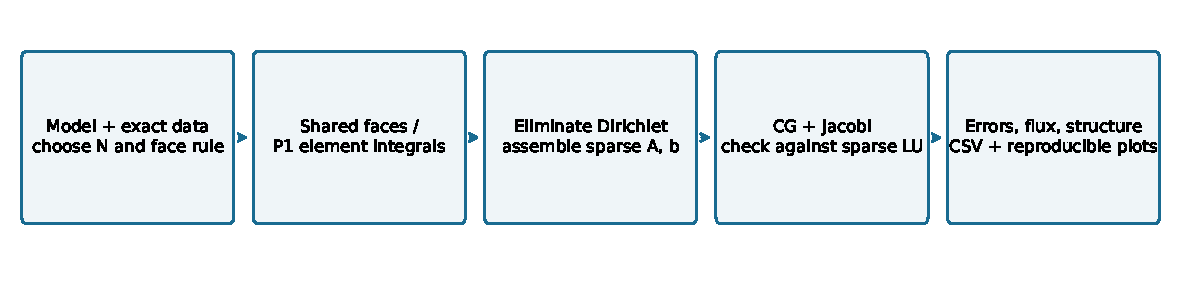
\includegraphics[width=\linewidth]{figures/fig01_algorithm.pdf}
\caption{Computational path from the continuous data to independently checked numerical output. The direct solve and the iterative solve act on the same assembled matrix and right-hand side.}
\label{fig:alg_flow}
\end{figure}

\subsection{Data layout and conservative FDM assembly}
The unit square is divided into $N$ intervals per coordinate, with $h=1/N$ and $n=N-1$ interior points. The code uses \texttt{indexing='ij'} and C-order flattening, so
\[
k=(i-1)n+(j-1),\qquad 1\leq i,j\leq n.
\]
The $y$ coordinate varies fastest. East/west connections have offsets $\pm n$ and north/south connections have offsets $\pm1$. Separate two-dimensional masks define these connections, preventing a spurious wrap between adjacent grid columns.

Each physical edge coefficient is computed once. The smooth benchmark uses arithmetic averages of neighbouring nodal coefficients. The layered benchmark uses odd $N$ so the interface bisects an edge, and compares arithmetic against harmonic averages. After division by $h^2$, the same edge weight is inserted into the two transposed off-diagonal positions. The diagonal retains all four outgoing weights. A boundary neighbour contributes $+a_fg/h^2$ to the right-hand side. Only interior unknowns enter the matrix.

\begin{algorithm}[H]
\caption{Vectorised conservative FDM assembly}
\begin{algorithmic}[1]
\Require $N$, coefficient and source functions, Dirichlet data, face rule
\Ensure Interior CSR matrix $A$ and right-hand side $b$
\State Sample $a$, $f$ and $g$ on the prescribed grid
\State Form shared $x$-edge and $y$-edge coefficients
\State Form the $(N-1)\times(N-1)$ interior index array
\State Add the diagonal sum of four face weights
\State Add each interior connection in both matrix directions
\State Add known boundary contributions to $b$
\State Construct COO arrays and convert to CSR
\State Check symmetry, diagonal signs and off-diagonal signs
\end{algorithmic}
\end{algorithm}

The exact FDM nonzero count is $5n^2-4n$, and assembly and matrix-vector products require $\mathcal O(n^2)$ storage and work. The unit test at $N=3$ checks the hand-derived $4\times4$ constant-coefficient matrix. A second test checks the coefficient $-N^2(20/11)$ in a row adjacent to the material interface. Together they check the ordering, scaling and special interface row.

\lstinputlisting[firstline=65,lastline=76,caption={The actual vectorised COO assembly in \texttt{src/discretisation.py}. Each interior connection contributes a symmetric pair.}]{src/discretisation.py}

\begin{figure}[H]
\centering
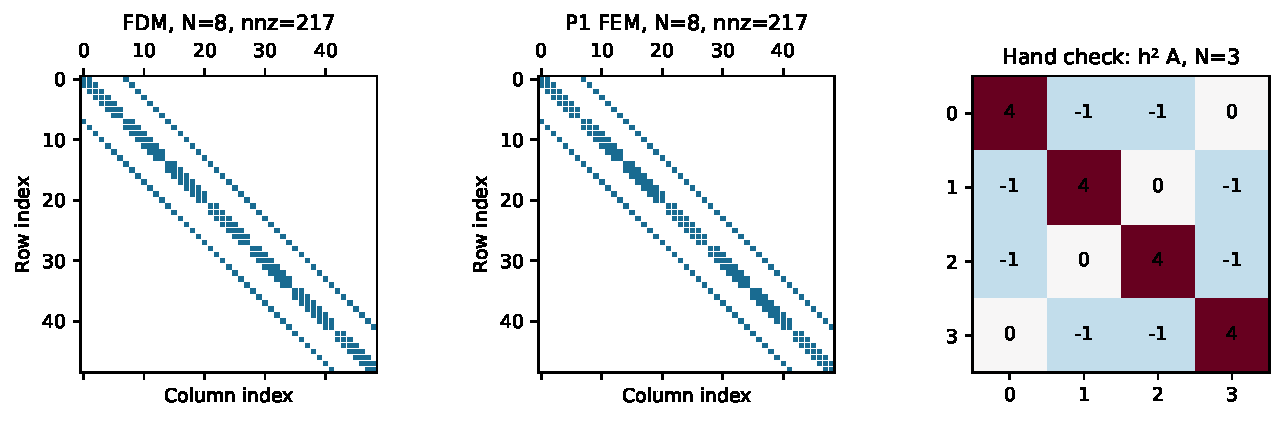
\includegraphics[width=0.96\linewidth]{figures/fig02_sparse_assembly.pdf}
\caption{Actual matrix patterns and the hand-check matrix. With this right-triangle mesh, zero cross-diagonal element couplings are removed from sparse storage. Similar sparsity patterns alone do not establish equality of the FDM and FEM operators or loads.}
\label{fig:alg_spy}
\end{figure}

\subsection{Linear solvers, residuals and measured cost}
Symmetric Dirichlet elimination and positive conductances give the SPD structure required by conjugate gradients. The main comparison uses CG with zero initial guess and Jacobi inverse preconditioner $M=\operatorname{diag}(A)^{-1}$, with the same requested tolerance for both discretisations. SciPy's interface checks
\[
\|b-AU\|_2\leq\max(\mathrm{rtol}\|b\|_2,\mathrm{atol}),
\qquad \mathrm{rtol}=10^{-12},\quad\mathrm{atol}=0.
\]
The code explicitly recomputes the residual after CG exits. If round-off in the recursively updated residual leaves the recomputed residual above the target, it solves a residual-correction system and adds the correction. At most three corrections are allowed. The final explicit check permits a 10\% floating-point margin on the requested tolerance; failure raises an error. Correction iterations and work enter the reported CG totals.

A sparse SuperLU factorisation supplies an independent solution of the same system. The code calls \texttt{splu} on a CSC matrix with COLAMD ordering, then applies the factorisation to $b$. This separates factorisation from triangular-solve cost. It also reports
\[
\eta_\infty=
\frac{\|b-AU\|_\infty}{\|A\|_\infty\|U\|_\infty+\|b\|_\infty},
\qquad
\delta_{\rm alg}=\|U_{\rm CG}-U_{\rm LU}\|_\infty.
\]
The independent solution difference measures the solver contribution relative to the observed discretisation error. A small residual is supported by this solution check.

Assembly, preconditioner setup, CG, LU factorisation and triangular solves are timed separately with \texttt{perf\_counter}. Timings use three serial repetitions, and each reported stage is its median. Numerical thread pools are limited to one thread. Diagnostic residual histories, quadrature error evaluation, eigenvalue estimation, file writing and plotting lie outside the reported main-solve timings. The cost--accuracy plot uses assembly plus Jacobi setup plus CG. Environment versions, source hashes and all individual timing repetitions accompany the tables.

\subsection{Two-dimensional P1 FEM and matched settings}
Each Cartesian square is split along the lower-left to upper-right diagonal. Three vertex indices describe each triangle. The constant local basis gradients are obtained from the affine triangle map, and the code assembles
\[
K_{ij}^{T}=(\nabla\varphi_i\cdot\nabla\varphi_j)\int_T a\,dx,
\qquad b_i^T=\int_Tf\varphi_i\,dx.
\]
This implementation uses explicit NumPy element arrays and SciPy assembly. A $5\times5$ Gauss--Legendre rule under a Duffy map evaluates the triangle integrals. With reference coordinates $r,s\in(0,1)$, the barycentric coordinates are $((1-r)(1-s),r,(1-r)s)$ and the Jacobian factor is $1-r$. The reference weights sum to $1/2$. For the affine smooth coefficient and for an aligned piecewise-constant coefficient, this rule integrates stiffness coefficients exactly up to round-off. A higher quadrature order independently checks the smooth load and error integral on a representative mesh.

Local $3\times3$ matrices are accumulated in COO format, converted to CSR and duplicate entries summed. With boundary vertex set $B$ and interior set $I$, Dirichlet data are imposed through
\[
K_{II}U_I=b_I-K_{IB}g_B.
\]
The raw FEM flux is $-a\nabla u_h$ on each triangle. Its one-sided normal traces are evaluated from the actual neighbouring elements. Conforming P1 functions are continuous, while their raw normal fluxes generally jump. The particular aligned layered solution belongs to the finite-element space, permitting a separate exactness check.

The smooth comparison uses $N=16,32,64,128$, identical data, common vertices, identical CG stopping settings, and the same Jacobi construction. Each method has $(N-1)^2$ unknowns. The named nodal errors are
\[
E_{2,h}=h\left(\sum_{i,j\in I}|U_{ij}-u_*(x_i,y_j)|^2\right)^{1/2},
\qquad E_\infty=\max_{i,j}|U_{ij}-u_*(x_i,y_j)|.
\]
The code additionally evaluates a common continuous $L^2$ error. Both nodal solutions are reconstructed using P1 interpolation on the same triangles and integrated against the exact solution with a $6\times6$ Duffy quadrature rule. This explicitly defines how a nodal FDM solution enters a continuous-norm comparison. Successive-grid rates use the actual ratio of mesh widths; fitted rates use the last three meshes.

For the layered structural check, FDM uses $N=31,63,127,255$, while interface-fitted FEM uses $N=32,64,128,256$. This parity difference is recorded in the data. The smooth experiment supplies the equal-mesh accuracy comparison.

\subsection{Verification evidence produced by the implementation}
Seven automated tests cover the hand matrix and special row, independent manufactured forcing, layered exactness and matrix structure, smooth convergence and quadrature, an affine FEM patch, the arithmetic comparison with parity checks, and the explicit CG residual with direct-solution agreement. An independent centred difference of the analytical flux verifies the manufactured source. The layered tests check the exact solution, interface flux, symmetry, positive smallest eigenvalue on a small matrix, and bounds on the solution.

On the smooth representative mesh $N=32$, the tolerance sweep keeps $A$ and $b$ fixed while changing CG rtol from $10^{-6}$ to $10^{-9}$ and $10^{-12}$. Table~\ref{tab:alg_tol} displays the algebraic difference and total nodal error separately. The main four-mesh experiment also checks $\delta_{\rm alg}/E_\infty<10^{-3}$ at every level.

\begin{table}[H]\centering\small
\begin{tabular}{lrrrr}
\toprule
Method & CG rtol & $\|U_{\rm CG}-U_{\rm LU}\|_\infty$ & $E_\infty$ & $\|r\|_2/\|b\|_2$\\
\midrule
FDM & 1e-06 & 5.810e-10 & 8.009e-04 & 1.133e-07\\
FDM & 1e-09 & 4.033e-12 & 8.009e-04 & 8.193e-10\\
FDM & 1e-12 & 5.329e-15 & 8.009e-04 & 8.071e-13\\
FEM & 1e-06 & 3.995e-08 & 8.079e-04 & 7.398e-07\\
FEM & 1e-09 & 8.902e-11 & 8.079e-04 & 7.270e-10\\
FEM & 1e-12 & 1.010e-14 & 8.079e-04 & 5.540e-13\\
\bottomrule
\end{tabular}

\caption{Actual tolerance sweep on the same smooth problem at $N=32$. Errors and residuals are recomputed after the solve.}
\label{tab:alg_tol}
\end{table}

\begin{figure}[H]\centering
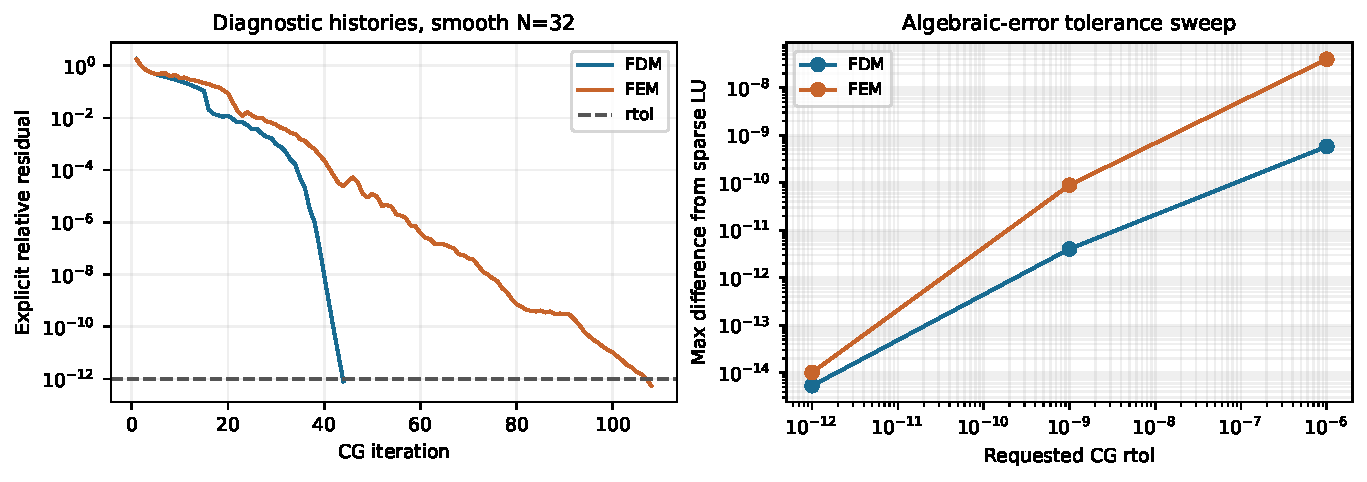
\includegraphics[width=0.95\linewidth]{figures/fig06_solver_validation.pdf}
\caption{Explicit residual histories and solution agreement with the direct reference. History collection performs additional matrix-vector products and is excluded from the main timing comparison.}
\end{figure}

\begin{table}[H]\centering\small
\begin{tabular}{llrrrrr}
\toprule
Method & $N$ & DOF & $E_{2,h}$ & $E_\infty$ & $p_{2,h}$ & CG its.\\
\midrule
FDM & 16 & 225 & 1.598e-03 & 3.205e-03 & --- & 19\\
FDM & 32 & 961 & 3.988e-04 & 8.009e-04 & 2.00 & 44\\
FDM & 64 & 3969 & 9.966e-05 & 2.003e-04 & 2.00 & 94\\
FDM & 128 & 16129 & 2.491e-05 & 5.007e-05 & 2.00 & 192\\
FEM & 16 & 225 & 1.614e-03 & 3.214e-03 & --- & 53\\
FEM & 32 & 961 & 4.042e-04 & 8.079e-04 & 2.00 & 108\\
FEM & 64 & 3969 & 1.011e-04 & 2.021e-04 & 2.00 & 225\\
FEM & 128 & 16129 & 2.527e-05 & 5.053e-05 & 2.00 & 443\\
\bottomrule
\end{tabular}

\caption{Computed four-mesh validation for both implementations. $p_{2,h}$ is the successive-grid rate in the nodal area-weighted norm. The CSV also contains continuous reconstructed errors, maximum-norm rates and residuals.}
\label{tab:alg_smooth}
\end{table}

\begin{figure}[H]\centering
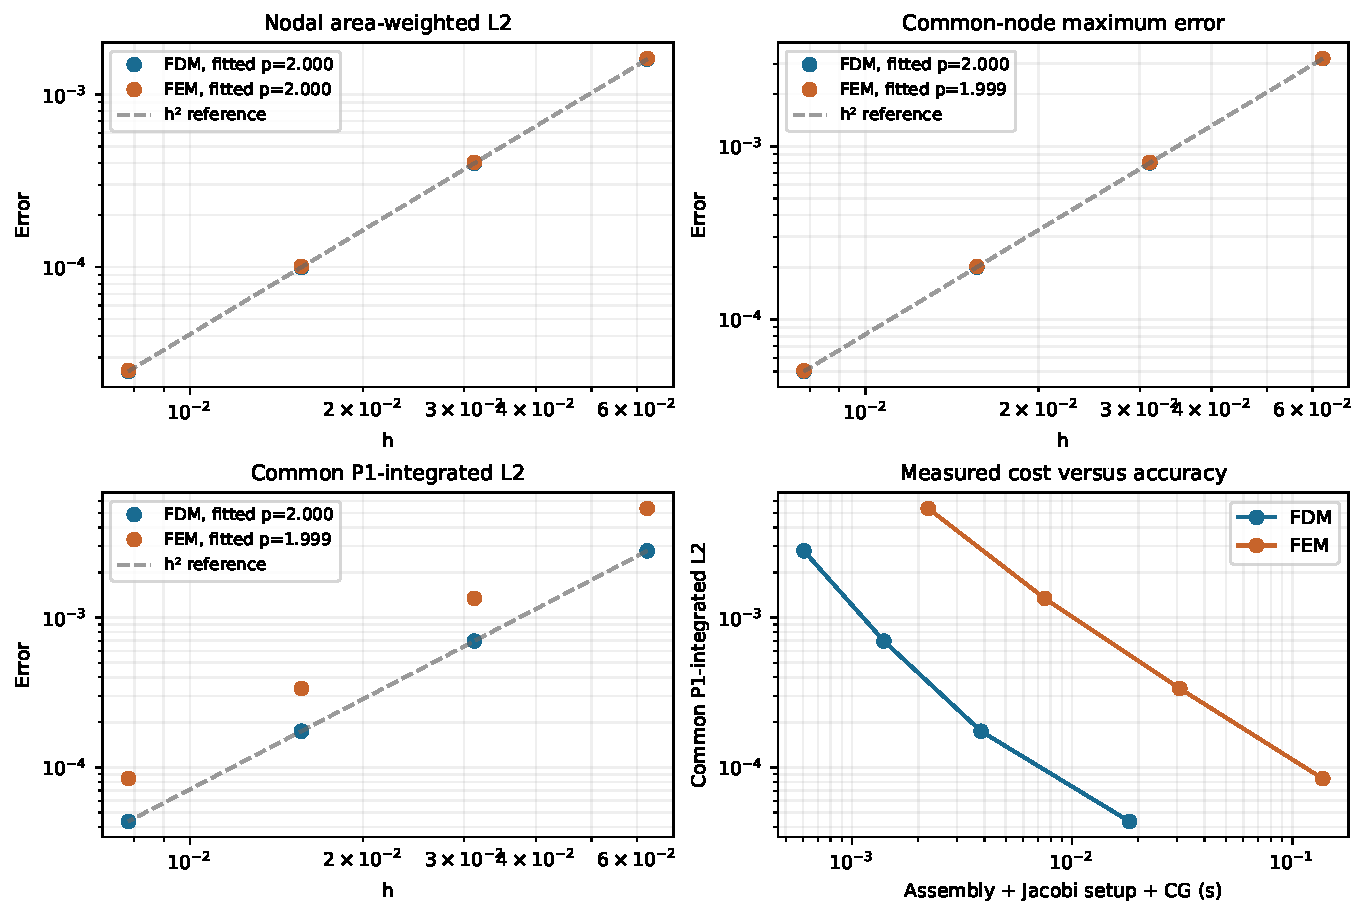
\includegraphics[width=0.91\linewidth]{figures/fig03_accuracy_cost.pdf}
\caption{Refinement checks in two nodal norms and a common integrated norm, with the measured assembly-and-CG cost. Fitted orders use the finest three meshes; the dashed lines show the theoretical quadratic slope. Timings are local CPU measurements.}
\end{figure}

\begin{table}[H]\centering\small
\begin{tabular}{lrrrrr}
\toprule
Method & $N$ & nnz & Assembly (s) & CG (s) & LU (s)\\
\midrule
FDM & 64 & 19593 & 8.243e-04 & 2.890e-03 & 6.199e-03\\
FDM & 128 & 80137 & 2.738e-03 & 1.528e-02 & 3.059e-02\\
FEM & 64 & 19593 & 2.409e-02 & 6.675e-03 & 5.478e-03\\
FEM & 128 & 80137 & 1.026e-01 & 3.474e-02 & 3.078e-02\\
\bottomrule
\end{tabular}

\caption{Median stage costs from three repetitions. CG excludes Jacobi setup in this table; LU includes factorisation and one triangular solve. The cost--accuracy plot additionally includes assembly and Jacobi setup.}
\end{table}

\subsection{Interface diagnostics and coefficient contrast}
All fluxes use the common $+x$ normal and the physical sign $q_x=-a\partial_xu$. For FDM the code forms the shared edge fluxes directly from the face arrays. Their discrete divergence checks the assembled local balance. The interface flux error is measured against $q_*=-2c/(1+c)$. To quantify a two-sided flux difference, the code also evaluates the nearest pure-material edge on each side and reports the maximum difference at common $y$ values. These two edges are a distance $h$ apart from the interface. This reconstruction is exact for the piecewise-linear benchmark, and its location is explicit in the implementation.

The arithmetic scheme retains shared-face conservation. Its inaccurate interface resistance can alter the numerical solution and physical flux. The plots and data report the actual errors. The magnitude of a reconstructed jump depends on the reconstruction and boundary data. The raw FEM traces are evaluated on the two triangles adjacent to each aligned interface segment, sorted by segment midpoint.

In this experiment the arithmetic scheme also gives a very small two-sided reconstructed jump, while its shared interface flux has a substantial error against the exact flux (Table~\ref{tab:alg_interface}). Checking the jump alone would therefore miss the interface resistance defect. Harmonic nodal exactness refers to nodal values; plain P1 interpolation across an unresolved interface introduces an additional interpolation error in a continuous norm.

\begin{table}[H]\centering\small
\begin{tabular}{llrrrr}
\toprule
Method & Face rule & $N$ & $E_\infty$ & $E_q$ & $J_q$\\
\midrule
FDM & arithmetic & 63 & 9.600e-03 & 6.619e-01 & 3.846e-13\\
FDM & harmonic & 63 & 7.327e-15 & 1.081e-13 & 6.015e-13\\
FEM & element integral & 64 & 2.687e-14 & 4.456e-13 & 3.979e-13\\
\bottomrule
\end{tabular}

\caption{Layered diagnostics at neighbouring mesh sizes, $c=10$. $E_q$ is the maximum interface flux error; $J_q$ is the explicitly defined two-sided flux difference. Mesh parity follows each method's interface treatment.}
\label{tab:alg_interface}
\end{table}

\begin{figure}[H]\centering
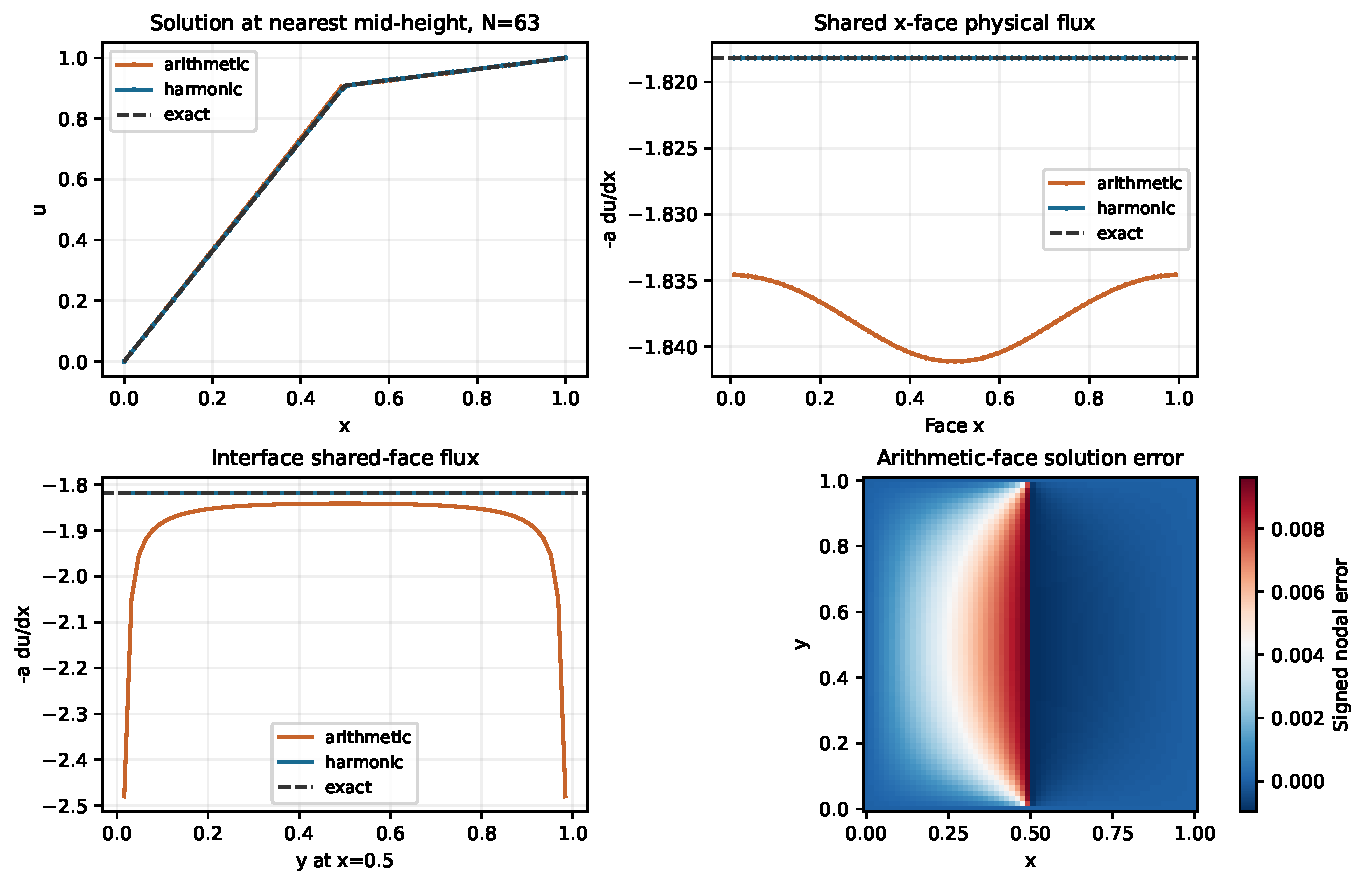
\includegraphics[width=0.90\linewidth]{figures/fig04_interface.pdf}
\caption{Computed layered FDM fields at $N=63$. The lower-left panel displays the shared interface flux along $y$, with prescribed top and bottom boundary edges excluded. The error map shows how an interface conductance defect affects the two-dimensional solution.}
\end{figure}

For conditioning, the harmonic FDM matrix is tested at $N=15,31,63$ and $c=1,10,100$. The smallest eigenvalue is estimated using shift-invert Lanczos with shift zero; the largest uses the largest-algebraic option. The reported estimate is $\widehat\kappa_2=\widehat\lambda_{\max}/\widehat\lambda_{\min}$. Explicit eigenpair residuals accompany each estimate. CG iteration counts are recorded with and without Jacobi at comparable explicit relative residuals. These data concern the unscaled Dirichlet-eliminated FDM matrix. The analytical contrast-dependent bound remains an upper bound; the experiments measure the behaviour for this coefficient geometry.

\begin{figure}[H]\centering
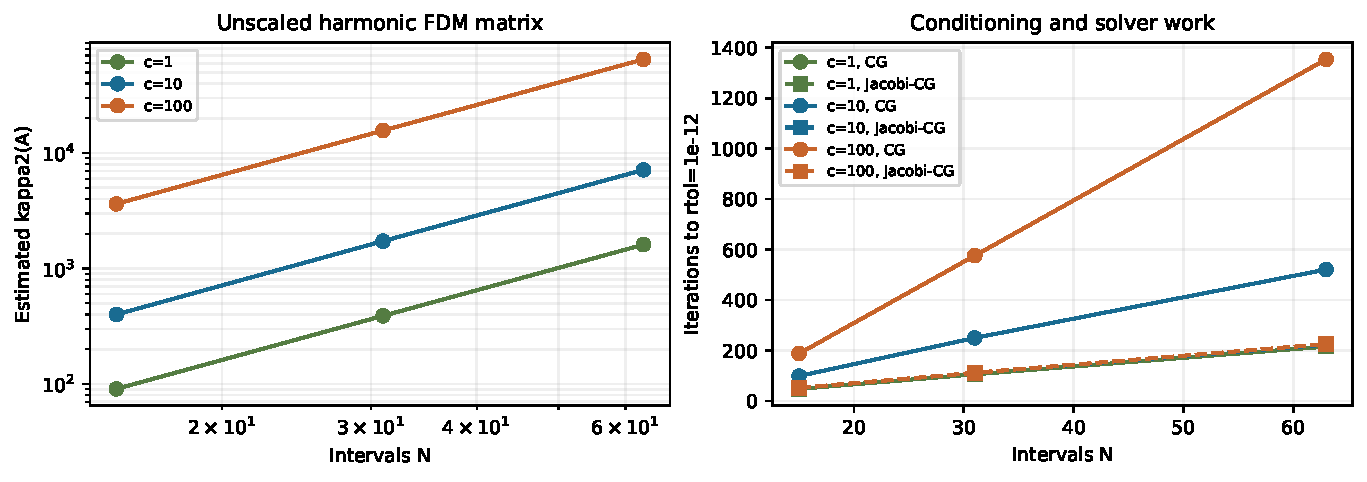
\includegraphics[width=0.95\linewidth]{figures/fig05_conditioning.pdf}
\caption{Estimated conditioning and actual CG work under mesh refinement and coefficient contrast. Jacobi changes the iterative system, while the left panel always refers to the original matrix.}
\end{figure}

\subsection{Reproduction and integration}
\texttt{python -B run\_all.py} reruns the checks, numerical experiments, tables and six figures from the configuration file. The implementation uses double precision. The supplied PDF is a standalone reading version; \texttt{algorithm\_section.tex} can be included as Section~3 after the supplied Method section. The folder contains the numerical source, tests, raw CSV tables, representative field arrays, figures in PDF/PNG, and software provenance. The existing interface-PINN experiment is available as a separate advanced supplement, with its own training outputs and architecture limitations.

\newpage
\section{Verification and Numerical Experiments}
\label{sec:results}

This section interprets the saved measurements from the pinned Project 2
repository. The core method is the conservative FDM; the conforming
$\mathcal P_1$ FEM supplies the required depth comparison. All reported
errors use the exact benchmark solutions specified in the problem pack
\cite{problempack}. The input data, assembly, solver, and post-processing
definitions are given in Sections~2--3.

\subsection{Checks before interpreting error tables}
The smooth forcing was derived analytically from
$u_*=\sin(\pi x)\sin(\pi y)$ and $a=1+x$. An independent derivative check in
the validation suite found a maximum absolute source defect of
$7.11\times10^{-15}$ in its complex-step comparison. An affine patch with
asymmetric nonzero values on all four sides gave a maximum difference of
$4.89\times10^{-15}$ between the production boundary elimination and an
independently assembled dense reference. These checks probe the source sign,
index ordering, and Dirichlet right-hand side rather than merely reproducing
the same code path.

For the smooth $N=32$ FDM and FEM systems, the tolerance sweep in
Table~\ref{tab:alg_tol} uses the same assembled matrix and right-hand side at
each solver tolerance. Tightening the requested CG relative residual from
$10^{-6}$ to $10^{-12}$ changed the CG--LU maximum solution difference from
$5.81\times10^{-10}$ to $5.33\times10^{-15}$ for FDM and from
$4.00\times10^{-8}$ to $1.01\times10^{-14}$ for FEM. Both values at the
tightest setting lie far below the approximately $8\times10^{-4}$ nodal
discretisation error. Across all four smooth levels, the recorded
algebraic-to-discretisation error ratio remained below $10^{-3}$.

The assembled FDM matrices have zero measured relative symmetry defect in
the saved runs, positive diagonals, non-positive off-diagonals, and positive
smallest eigenvalues in the independently checked small and medium systems.
The energy identity in Theorem~\ref{thm:spd_mmatrix} is the proof of positive
definiteness; an eigensolver estimate is corroboration. The layered solutions
stay within the prescribed boundary range $[0,1]$. This supports the
discrete maximum-principle prediction, although it says nothing about the
accuracy of the interface resistance.

\subsection{Smooth coefficient: convergence and method comparison}
Table~\ref{tab:alg_smooth} reports four refinements for both discretisations,
with $N=16,32,64,128$ and $225$ to $16\,129$ unknowns. At the finest level,
FDM gives $E_{2,h}=2.491\times10^{-5}$ and
$E_\infty=5.007\times10^{-5}$; FEM gives
$2.527\times10^{-5}$ and $5.053\times10^{-5}$ in the same nodal norms.
The independent validation fit over $N=32,64,128$ is $2.00034$ for FDM and
$1.99964$ for FEM in $E_{2,h}$. For the common reconstructed continuous
$L^2$ norm, the corresponding fits are $1.99996$ and $1.99898$. The observed
orders therefore match the second-order prediction on this smooth problem.
The $a=1+x$ coefficient is affine, so arithmetic averaging equals exact
midpoint sampling; this benchmark does not test the distinct arithmetic
averaging error for a curved smooth coefficient.

The matched comparison uses the same square mesh, nodal data, number of
interior unknowns, CG stopping rule, and common reconstruction for continuous
$L^2$. At $N=128$, the latter error is $4.360\times10^{-5}$ for FDM and
$8.415\times10^{-5}$ for FEM. The two methods are both second order, but
their constants differ under this particular reconstruction and triangular
quadrature. The FEM's mathematical $L^2$ convergence rate and this measured
constant should not be conflated with its nodal error, which is much closer
to FDM's on this example.

The cost table in Section~3 reports local medians over three serial runs.
At $N=128$, FDM assembly took $2.74\times10^{-3}$ seconds and FEM assembly
$1.03\times10^{-1}$ seconds; the respective Jacobi-CG solves took
$1.53\times10^{-2}$ and $3.47\times10^{-2}$ seconds, with $192$ and $443$
iterations. The sparse LU solves were about $3.06\times10^{-2}$ and
$3.08\times10^{-2}$ seconds, respectively. Both matrices had $80\,137$
stored nonzeros after explicit zero removal. These timings are measurements
for the supplied implementations and hardware, not general speed constants
for FDM or FEM. The implemented FEM assembly performs element quadrature and
therefore has more work per unknown than this vectorised FDM assembly.

\subsection{Layered interface: accuracy, flux, and maximum principle}
For $a_L=1$ and $a_R=10$, the exact flux is $J_*=-20/11$. Odd FDM meshes
place the interface halfway between columns; even FEM meshes align it with
element edges. Table~\ref{tab:interface_refinement} extends the single-mesh
comparison of Table~\ref{tab:alg_interface} to all four odd FDM meshes.

\begin{table}[H]
\centering\small
\begin{tabular}{rrrrrr}
\toprule
$N$ & Rule & $E_{2,h}$ & $E_\infty$ & $E_q^{\max}$ & $E_q^{\mathrm{mid}}$\\
\midrule
31 & arithmetic & 6.767e-03 & 1.938e-02 & 6.629e-01 & 4.697e-02\\
31 & harmonic & 4.940e-16 & 1.443e-15 & 2.953e-14 & 1.088e-14\\
63 & arithmetic & 3.271e-03 & 9.600e-03 & 6.619e-01 & 2.294e-02\\
63 & harmonic & 1.747e-15 & 7.327e-15 & 1.081e-13 & 1.081e-13\\
127 & arithmetic & 1.607e-03 & 4.777e-03 & 6.616e-01 & 1.134e-02\\
127 & harmonic & 6.261e-15 & 1.399e-14 & 3.813e-13 & 7.372e-14\\
255 & arithmetic & 7.963e-04 & 2.383e-03 & 6.615e-01 & 5.641e-03\\
255 & harmonic & 1.085e-13 & 2.183e-13 & 4.696e-13 & 5.795e-14\\
\bottomrule
\end{tabular}

\caption{Independent layered FDM validation at contrast $c=10$.
$E_q^{\max}$ is the maximum error of the shared interface-face flux over the
interior face samples; $E_q^{\mathrm{mid}}$ is the error at the sample nearest
$y=1/2$. The harmonic method's nodal errors are at round-off.}
\label{tab:interface_refinement}
\end{table}

Harmonic FDM reproduces the nodal exact solution to a maximum error below
$2.2\times10^{-13}$ at all listed meshes. On $N=63$ the interface flux error
is $1.08\times10^{-13}$. The fitted FEM at $N=64$ likewise has a nodal
maximum error of $3.31\times10^{-14}$ and interface flux error
$5.17\times10^{-13}$. The P1 result is exact in this benchmark because the
piecewise-linear exact solution belongs to the fitted finite-element space;
general P1 solutions need not have pointwise continuous element flux.

Arithmetic FDM gives $E_\infty=9.600\times10^{-3}$ at $N=63$, falling to
$2.383\times10^{-3}$ at $N=255$. Its successive measured nodal orders are
$0.991$, $0.995$, and $0.998$, consistent with first-order convergence in
this test. The maximum shared interface-flux error, however, is approximately
$0.662$ on each mesh. The midline error decreases from $4.70\times10^{-2}$
at $N=31$ to $5.64\times10^{-3}$ at $N=255$. The maximum persists because
the top and bottom boundaries retain the prescribed exact trace while the
arithmetic interface resistance perturbs nearby interior nodes. Thus the
one-dimensional resistance calculation in Section~2 predicts the wrong
conductance but does not describe the maximum face-flux error on the
two-dimensional Dirichlet square.

The arithmetic matrix is still symmetric and conserves one shared face flux
between adjacent cells. At $N=63$, the two-sided reconstructed flux
difference at the nearest pure-material edges is only
$3.85\times10^{-13}$, while the interface flux is wrong by $0.662$ at its
worst sample. This illustrates why a small reconstructed jump or a matrix
symmetry check cannot by itself validate physical interface accuracy. Both
arithmetic and harmonic solutions remain in $[0,1]$, as predicted by their
common positive-face M-matrix structure.

\subsection{Mesh size, contrast, and iterative work}
Table~\ref{tab:conditioning_corrected} uses the independent spectral
validation record. The original condition-number diagnostic used a fixed
structured Lanczos start that missed the largest eigenvalue when $c=1$;
the independent calculation used an alternative start and checked the
constant-coefficient formula. The $c=10$ and $c=100$ entries agreed with
the repository's estimates to reported precision.

\begin{table}[H]
\centering\small
\begin{tabular}{rrrrr}
\toprule
$N$ & $c$ & $\kappa_2(A_h)$ & CG iterations & Jacobi--CG iterations\\
\midrule
15 & 1 & 9.052e+01 & 48 & 48\\
31 & 1 & 3.888e+02 & 106 & 106\\
63 & 1 & 1.608e+03 & 216 & 216\\
15 & 10 & 3.996e+02 & 99 & 52\\
31 & 10 & 1.726e+03 & 250 & 112\\
63 & 10 & 7.149e+03 & 521 & 224\\
15 & 100 & 3.628e+03 & 188 & 52\\
31 & 100 & 1.567e+04 & 576 & 112\\
63 & 100 & 6.490e+04 & 1354 & 226\\
\bottomrule
\end{tabular}

\caption{Condition number and CG iterations for harmonic FDM under mesh
refinement and contrast. Residual tolerance is $10^{-12}$; the spectral
estimates use the independently checked largest eigenvalue.}
\label{tab:conditioning_corrected}
\end{table}

At $N=63$, raising contrast from $1$ to $10$ to $100$ raises the measured
condition number from about $1.61\times10^3$ to $7.15\times10^3$ to
$6.49\times10^4$. Unpreconditioned CG iterations rise from $216$ to $521$
to $1354$. With Jacobi scaling the corresponding counts are $216$, $224$,
and $226$. At fixed contrast, refinement also increases the condition
number, consistent with the $O(h^{-2})$ upper bound. These results support
the solver choice and show the practical value of preconditioning for this
layered geometry; they do not claim contrast-independent performance for
arbitrary heterogeneous media.


\section{Conclusions}
The conservative FDM correctly represents the divergence-form diffusion
operator when adjacent rows share each positive face conductance and
Dirichlet data are eliminated symmetrically. Its discrete energy identity
establishes positive definiteness, and its M-matrix sign pattern gives a
maximum principle. The smooth manufactured benchmark, independently
checked source term, four-level error table, and algebraic tolerance sweep
support approximately second-order accuracy for $a=1+x$.

The layered test separates algebraic structure from physical accuracy.
Harmonic averaging reproduces the piecewise-linear exact solution and
constant flux at the nodes and faces to round-off. Arithmetic averaging
retains symmetry, local discrete conservation, and the maximum principle,
yet its nodal error is first order and its maximum interface-flux error
stays near $0.662$ for the tested two-dimensional boundary data. A single
flux-jump statistic would have hidden this defect.

The matched FEM comparison gives the same approximately second-order order
on the smooth problem, with different measured constants and costs. The
fitted layered FEM is also exact for this particular solution. Contrast
increases the unscaled FDM condition number and unpreconditioned CG work;
Jacobi substantially reduces the contrast effect in the tested sequence.

The experiments are limited to a Cartesian square, a smooth affine
coefficient, and a straight two-material interface. Curved interfaces,
non-affine smooth coefficients, and general heterogeneous patterns require
separate verification. The supplied code and raw data permit the reported
tables and figures to be regenerated. Individual contribution statements
must be supplied by the team members from their own records.


% ---- Appendices -------------------------------------------------------
% Part A (team AI transparency log) and Part B (individual contribution
% statement) live in ics/MeichendingICS.tex, which is also the body of the
% standalone document project2/ics/MeichendingICS.tex. \reportbuild makes the
% cross-references in that file resolve to this report's numbers.
\def\reportbuild{}
\appendix
% ============================================================
% ICS & AI Transparency Log --- Meichen Ding (2362344)
%
% This file is the single source for two deliverables:
%   (a) Appendix A of project2/meichending/Method.tex, where it is included
%       after \appendix with \def\reportbuild{} set beforehand, so that the
%       cross-references resolve to the numbers of that report;
%   (b) the standalone document project2/ics/MeichendingICS.tex, which inputs
%       this file without \reportbuild, so the same sentences appear with
%       words instead of numbers.
% Format follows Checklist/ICS_bvp.tex: Part A is the team AI transparency
% log, Part B is the individual contribution statement.
% ============================================================

% Cross-reference helper. In the report build the numbered objects exist and
% are printed; in the standalone ICS document they do not, so plain words are
% printed instead and the document has no unresolved references.
\ifdefined\reportbuild
  \newcommand{\reftext}[2]{#1}
\else
  \newcommand{\reftext}[2]{#2}
\fi

\section{AI Transparency Log}
\label{app:ai_log}

This appendix records the distance between raw generative-AI output and the
claims that survived into this report; it is a record of auditing, not a count
of prompts. Every claim listed in A2 was re-derived, re-run against the team's
own code, or falsified before it was allowed into the text, and each of the
three audits changed a claim that an earlier draft had already stated. The
conversation transcripts are retained by the team and can be supplied on
request; they are not appended here.

\subsection*{A1. AI tools used}

\begin{table}[H]
\centering\small
\caption{Generative-AI tools used in Project 2. Entries describe the use that
actually reached the report; routine autocomplete and spelling checks are
covered by the last row.}
\label{tab:ai_tools}
\begin{tabular}{@{}>{\raggedright\arraybackslash}p{3.9cm}>{\raggedright\arraybackslash}p{3.3cm}>{\raggedright\arraybackslash}p{7.4cm}@{}}
\toprule
Tool & Version / date & Primary use \\
\midrule
DeepSeek-based assistant in DeepSeek Harness (\texttt{deepseek-flash})
  & current build, Oct--Nov 2026
  & Drafting and re-deriving \S1.2 and \S2.1--\S2.4 (model, weak form,
    truncation error, interface conductance, boundary elimination, discrete
    structure); writing the independent verification scripts in
    \path{support/verify/}; adversarial review of the section text. \\
Claude (Anthropic), web application
  & current build, Oct--Nov 2026
  & Drafting of the algorithm section, integration notes for merging the
    section files, figure and table captions, wording and consistency passes. \\
ChatGPT (OpenAI) and Gemini (Google)
  & current builds, Oct--Nov 2026
  & \LaTeX{} error diagnosis, document structure, phrasing and completeness
    checks. \\
\midrule
All of the above, routine use
  & ---
  & Autocomplete, spelling, reference formatting, table alignment. No numerical
    value was accepted without reproduction (see A3). \\
\bottomrule
\end{tabular}
\end{table}

\subsection*{A2. Significant AI-assisted claim audits}

Three interactions are recorded below because each one changed a mathematical
or numerical claim rather than simply rewording it. The common failure pattern
is a claim that is true for the face coefficient, or for one dimension, being
silently promoted to the solution of the two-dimensional problem.

{\footnotesize
\begin{longtable}{@{}p{0.95cm}>{\raggedright\arraybackslash}p{7.4cm}>{\raggedright\arraybackslash}p{5.8cm}@{}}
\caption{Claim audits. Column 3 states what would have shown the claim to be wrong.}\label{tab:ai_audits}\\
\toprule
Item & Prompt / claim / assumptions & Risk and possible falsifier \\
\midrule
\endfirsthead
\caption[]{Claim audits (continued).}\\
\toprule
Item & Prompt / claim / assumptions & Risk and possible falsifier \\
\midrule
\endhead
\bottomrule
\endfoot

1 &
``Arithmetic averaging of the interface conductance produces an
$\mathcal{O}(1)$ error in the interface flux, so the arithmetic-averaged
solution is $\mathcal{O}(1)$ inaccurate.''
\textbf{Assumption hidden in the wording:} the face-coefficient error and the
error of the discrete solution are the same object. &
The claim mixes three different quantities: the relative face-conductance
error $(1-c)^2/(4c)$ (genuinely $\mathcal{O}(1)$ in $h$), the nodal error and
the midline interface-flux error (first order in $h$), and the \emph{maximum}
interface-flux error over the square, which is $\mathcal{O}(1)$ for a different
reason --- the exact Dirichlet trace on $y=0,1$. \textbf{Falsifier:} a
refinement study. If the nodal error did not halve under mesh refinement, the
first-order part of the claim would be wrong. \\
2 &
``Since $A_h \succeq a_{\min}A_h^{(1)}$ in the Loewner order and both matrices
are $M$-matrices, the inverses compare entrywise,
$A_h^{-1}\le a_{\min}^{-1}(A_h^{(1)})^{-1}$; hence
$\|A_h^{-1}\|_\infty\le 1/(8a_{\min})$.'' \textbf{Assumption hidden:}
spectral order implies entrywise order. &
The implication is false: monotonicity of $M$-matrix inverses needs an
\emph{entrywise} hypothesis, while growing $a$ makes the off-diagonals
$-a_f/h^2$ \emph{more negative}. \textbf{Falsifier:} evaluate both inverses for
a strongly varying coefficient, e.g.\ $a=1+9\sin^2(\pi x)$ at $n=63$, where the
entrywise ratio reaches $3.10>1$. The conclusion
$\|A_h^{-1}\|_\infty\le1/(8a_{\min})$ is nevertheless true and is therefore
proved by a maximum-principle barrier argument instead. \\
3 &
``The arithmetic operator is symmetric and its shared face flux is
conservatively balanced, so the interface physics is correct.'' &
Symmetry and local conservation are necessary but not sufficient; they are
satisfied by a matrix whose interface flux is wrong by $36\%$.
\textbf{Falsifier:} compare the computed interface flux with the exact
$J_*=-20/11$ on a benchmark whose exact solution is known. It differs by
$0.662$ while the two-sided reconstructed jump is $3.85\times10^{-13}$ and the
symmetry defect is zero. \\
\end{longtable}}


\subsection*{A3. Independent verification and decision}

{\footnotesize
\begin{longtable}{@{}p{0.95cm}>{\raggedright\arraybackslash}p{6.2cm}>{\raggedright\arraybackslash}p{7.0cm}@{}}
\caption{What was checked, where the evidence lives, and what changed.}\label{tab:ai_verification}\\
\toprule
Item & Independent check and evidence location & Final decision / modification / limitation \\
\midrule
\endfirsthead
\caption[]{Independent verification (continued).}\\
\toprule
Item & Independent check and evidence location & Final decision / modification / limitation \\
\midrule
\endhead
\bottomrule
\endfoot

1 &
Re-derived the truncated-series argument in one dimension, where the discrete
system reduces to a tridiagonal chain with a closed-form flux; reproduced the
leading term $h(a_L-a_R)^2/(a_L+a_R)^2$ analytically and confirmed it against
$N=31,\dots,255$ (\path{support/verify/check_interface_order.py},
\reftext{Table~\ref{tab:interface_refinement}}{\S4.3}). Then re-assembled the
full two-dimensional layered problem and compared the nodal, midline and
maximal face-flux errors with \S4.3. &
The two-layer statement of \S2.2 and
\reftext{Remark~\ref{rem:arith_2d_boundary}}{the remark on the two-dimensional
boundary} replaced the single blanket $\mathcal{O}(1)$ claim: first-order nodal
and midline flux error, $\mathcal{O}(1)$ maximal face-flux error near the
prescribed horizontal boundaries, $\mathcal{O}(1)$ face-conductance error.
\textbf{Limitation:} the maximum is a boundary effect of the Dirichlet square;
it is stated as an observation on this benchmark, not as an estimate valid for
other boundary data. \\
2 &
Ran the counterexample search and the bound check in
\path{support/verify/check_stability.py}: entrywise ratio for
$a=1+9\sin^2(\pi x)$, $\|A_h^{-1}\|_\infty$ against $1/(8a_{\min})$ for five
coefficients in one and two dimensions, and the comparison with the
constant-coefficient maximum $0.0736<\frac18$
(\reftext{Remark~\ref{rem:entrywise_false}}{the remark recording the
counterexample}, \reftext{Remark~\ref{rem:conv_constant}}{the remark on the
constant}). &
The proof of \reftext{Theorem~\ref{thm:convergence}}{the convergence theorem}
was rewritten with a maximum-principle barrier: $A_h\bm\varphi=\bm 1$ exactly
for $\varphi=\frac12x(1-x)/a_{\min}$ extended by its own boundary values, and
$A_h(\bm\varphi-\bm w)=0$ with $\bm\varphi-\bm w\ge0$ on $\partial\Omega$.
\textbf{Limitation:} equality in $\|\bm w\|_\infty\le1/(8a_{\min})$ holds only
in one dimension; in two the constant is an upper bound ($0.0736$ versus
$0.125$). \\
3 &
Separated the three diagnostics on the same computed solution: symmetry defect
$\|A_h-A_h^T\|/\|A_h\|$, reconstructed two-sided flux jump, and error against
the exact flux
(\reftext{\S\ref{sec:results}}{\S4} and the interface diagnostics of
\reftext{\S\ref{sec:algorithm_impl}}{\S3}; independent re-computation in
\path{test/validate_interface.py}). &
\reftext{Remark~\ref{rem:symmetry_vs_accuracy}}{The remark on symmetry versus
accuracy} and \S4.3 now report the three numbers side by side instead of
treating symmetry as evidence of physical accuracy. \textbf{Limitation:} the
jump diagnostic is only defined where a two-sided reconstruction exists, so it
is not a substitute for an exact solution. \\
\end{longtable}}


Two further routine checks are recorded for completeness. The smooth benchmark
is \emph{blind} to the $\theta$-correction of the face coefficient when
$a=1+x$: arithmetic and midpoint averaging then produce entrywise identical
matrices, so the second-order table in \S4.2 cannot validate the correction
term (\reftext{Remark~\ref{rem:theta_blind}}{the remark on the
$\theta$-correction}). And no convergence claim is made anywhere in this report
without a named norm and a four-level refinement table; claims about the
layered benchmark are exactness statements
(\reftext{Theorem~\ref{thm:nodal_exactness}}{the nodal-exactness theorem}), not
order statements, because $u_*\notin H^2(\Omega)$ there
(\reftext{Remark~\ref{rem:thm2_scope}}{the remark on the validity of the
truncation analysis}).

\subsection*{A4. Intellectual ownership declaration}

The mathematical formulation, the discretisation, the solvers, the experiments,
the validation evidence and the conclusions are the team's own work.
Generative AI was used for drafting, clarification and preliminary checking, and
every AI-assisted claim was audited as recorded above. Each member affirms that
they can explain and modify the team-owned discretisation and solver code,
justify the mathematical claims in their own sections, and state the
assumptions and the tests applied at each library interface, without AI
assistance during the viva. The viva may ask for a small live modification or
diagnostic on team-owned work.

\begin{table}[H]
\centering\small
\caption{Ownership declaration. This copy carries the signature of Meichen
Ding; the other four rows are completed and signed by each member in their own
copy of this table. A declaration is never drafted on another member's
behalf.}
\label{tab:ai_ownership}
\begin{tabular}{@{}>{\raggedright\arraybackslash}p{2.7cm}p{1.7cm}>{\raggedright\arraybackslash}p{4.9cm}>{\raggedright\arraybackslash}p{4.6cm}@{}}
\toprule
Name & Signature & Team-owned artefact / contribution & Trusted dependency and interface \\
\midrule
Meichen Ding (2362344)
  & \underline{\hspace{1.2cm}}
  & \S1.2; \S2.1--\S2.4; the remarks on the $\theta$-correction, on mesh
    parity, on the two-dimensional boundary and on symmetry versus accuracy;
    Appendix~A; the scripts in \path{support/verify/}
  & \texttt{numpy.linalg} dense solves and
    \texttt{scipy.sparse.linalg.eigsh} used only for corroboration: checked
    against explicit residuals, against the exact layered solution and against
    a dense Cholesky factorisation \\
\bottomrule
\end{tabular}
\end{table}

\section{Individual Contribution Statement}
\label{app:ics}

Part A above is the team log. The statement below is individual: it states in
the first person what I did, and it cross-references the audits of
Section~\ref{app:ai_log} where the corresponding AI-assisted claim was checked.

\begin{formbox}\small
\textbf{Individual Contribution Statement --- Project 2 (PDE BVP)}

\textbf{Name:} Meichen Ding (2362344)

\textbf{Role this project:} Mathematical theory lead (consistency, adaptivity
and convergence): owner of the model formulation, the discrete scheme, its
truncation-error and interface analysis, and the discrete-structure results.

\textbf{The specific things I did this project:}
\begin{enumerate}[leftmargin=1.4em,itemsep=0.15em]
  \item
  Wrote \S1.2 and \S2.1--\S2.4 of the report's \path{Method.tex}: the continuous
  problem and its hypotheses, the flux-balance derivation that fixes
  one shared face coefficient per edge, the index map and block-tridiagonal
  structure of the assembled operator (with the non-zero count $5n^2-4n$), the
  symmetric Dirichlet elimination and the hand-computed $4\times4$ matrix at
  $n=2$ used as the small-case oracle, the layered exact solution, the
  second-order local truncation error with its $\theta$-correction, the
  series-resistance proposition for the interface conductance with the relative
  error $(1-c)^2/(4c)$, the SPD / $M$-matrix / discrete-maximum-principle
  theorem, and the discrete stability and $\mathcal{O}(h^2)$ convergence theorem
  with its maximum-principle barrier argument.
  \item
  Wrote the independent verification scripts \path{support/verify/}:
  \texttt{check\_interface\_order.py} (one-dimensional conservative scheme,
  $a_L=1$, $a_R=10$, $N=31,63,127,255$; harmonic nodes exact to $10^{-14}$ and
  every face flux equal to $-20/11$, arithmetic nodal error first order with
  measured orders $1.015/1.008/1.004$ and the closed-form chain flux
  reproduced), \texttt{check\_stability.py} (the entrywise-ratio counterexample
  at $a=1+9\sin^2(\pi x)$, ratio $3.10$; $\|A_h^{-1}\|_\infty$ against
  $1/(8a_{\min})$ for five coefficients) and
  \texttt{check\_matrix\_evidence.py} (symmetry defect, \texttt{eigsh} smallest
  eigenvalue and dense Cholesky on the submitted assembler). These produced the
  numbers in the appendix tables and in \S2.4.
  \item
  Ran the AI-assisted claim audits of Part A: the three-layer separation of the
  arithmetic-averaging errors (audit 1), the falsification of the
  Loewner-implies-entrywise argument and its replacement by the barrier proof
  (audit 2), and the separation of ``symmetric and conservative'' from
  ``physically correct'' (audit 3), including the numerical values that decide
  each one ($0.662$ versus $3.85\times10^{-13}$; $3.10>1$; $0.0736$ versus
  $0.125$).
\end{enumerate}

\textbf{What I would do differently:}
I would pin down the mesh convention with the code owner before writing any
convergence sentence. The skeleton uses $h=1/(n+1)$ with $n$ interior points
while the report uses $h=1/N$ with $N$ intervals, so the same symbol $N$ means
different things in the skeleton, in the layered tables and in the FEM
comparison; the interface-parity requirement $N$ odd for the FDM and $N$ even
for the FEM then has to be stated as design rather than discovered late. I would
also have demanded the two-dimensional layered numbers before writing the
one-dimensional flux estimate, because that is exactly where the two-layer
statement became necessary.

\textbf{Anything I should have asked for help with earlier:}
I should have asked, in Week 5, for each member to commit their own sections and
their own ICS from their own account. By the time the appendices were written
the repository history was a single upload commit, so authorship had to be
reconstructed from memory and from section ownership instead of being visible in
\texttt{git log}. I also should have asked for a review of the stability proof
before it went into a draft: the Loewner-order step survived an internal
re-reading and was only caught when it was written out as a counterexample
search.

\vspace{0.8em}
\textbf{Signature:} \underline{\hspace{5cm}} \hfill
\textbf{Date:} \underline{\hspace{3cm}}
\end{formbox}


\section{Reproducibility and Data Provenance}
\begin{sloppypar}
The supplied source package contains this report's \LaTeX{} sources, the
tables, the figures and the verification scripts; the FDM/FEM source and
\texttt{run\_all.py} are the team's, in \path{project2/algorithm_section/}. The snapshot is based on
\url{https://github.com/TTJTR/MTH321_TeamQ/tree/08bf8300e78c748fe5df0f1824d9780b6824446e/project2}.
The independent validation record is under \texttt{test/} in that snapshot. The
verification scripts quoted in Appendix~\ref{app:ai_log} are in
\texttt{support/verify/} and are independent of the production assembler:
\texttt{check\_interface\_order.py} re-derives the one-dimensional interface
numbers, \texttt{check\_stability.py} re-derives the discrete-stability
counterexample and the barrier bound, and \texttt{check\_matrix\_evidence.py}
regenerates Table~\ref{tab:matrix_evidence} from the submitted assembler.
The main results use double precision and the smooth and layered parameter
sets described in Sections~3--4. Timing values are local measurements and
will vary with hardware and software versions.
\end{sloppypar}

\bibliographystyle{plain}
\bibliography{refs}
\end{document}
